\documentclass[
% -- opções da classe memoir --
12pt,				% tamanho da fonte
oneside,			% para impressão em verso e anverso. Oposto a oneside
a4paper,			% tamanho do papel. 
% -- opções da classe abntex2 --
%chapter=TITLE,		% títulos de capítulos convertidos em letras maiúsculas
%section=TITLE,		% títulos de seções convertidos em letras maiúsculas
%subsection=TITLE,	% títulos de subseções convertidos em letras maiúsculas
%subsubsection=TITLE,% títulos de subsubseções convertidos em letras maiúsculas
% -- opções do pacote babel --
english,			% idioma adicional para hifenização
french,				% idioma adicional para hifenização
spanish,			% idioma adicional para hifenização
brazil				% o último idioma é o principal do documento
]{abntex2}

% ---
% Pacotes básicos 
% ---
\usepackage{pdfpages}
\usepackage{lmodern}			% Usa a fonte Latin Modern			
\usepackage[T1]{fontenc}		% Selecao de codigos de fonte.
\usepackage[utf8]{inputenc}		% Codificacao do documento (conversão automática dos acentos)
\usepackage{lastpage}			% Usado pela Ficha catalográfica
\usepackage{indentfirst}		% Indenta o primeiro parágrafo de cada seção.
\usepackage{color}				% Controle das cores
\usepackage{graphicx}			% Inclusão de gráficos
\usepackage{microtype} 			% para melhorias de justificação
\usepackage{float}
% ---
\usepackage{hyperref}

%\usepackage{titlesec}
\usepackage{titletoc}	



\usepackage{listings}
\usepackage{color}
\usepackage{lscape}

\definecolor{dkgreen}{rgb}{0,0.6,0}
\definecolor{gray}{rgb}{0.5,0.5,0.5}
\definecolor{mauve}{rgb}{0.58,0,0.82}


% ---
% Pacotes adicionais, usados apenas no âmbito do Modelo Canônico do abnteX2
% ---

% ---
% Pacotes de citações
% ---
\usepackage[brazilian,hyperpageref]{backref}	 % Paginas com as citações na bibl
\usepackage[alf]{abntex2cite}	% Citações padrão ABNT

\usepackage{xcolor}
% Definindo novas cores
\definecolor{verde}{rgb}{0.25,0.5,0.35}
\definecolor{jpurple}{rgb}{0.5,0,0.35}

\usepackage{listings}
\usepackage{multirow}
\usepackage{setspace}
\usepackage{lmodern} \normalfont %to load T1lmr.fd 

\usepackage{subcaption}
\usepackage{graphicx}


\DeclareFontShape{T1}{lmr}{bx}{sc} { <-> ssub * cmr/bx/sc }{}


\setlength{\parindent}{1.3cm}

% Controle do espaçamento entre um parágrafo e outro:
\setlength{\parskip}{0.2cm}  % tente também \onelineskip

\renewcommand{\appendixname}{Anexo}	

\newenvironment{citaçoes}{%
\begin{list}{}{%
	
}
\item\relax
}{\end{list}}


\renewcommand{\appendixname}{Anexo}	

\lstdefinelanguage{JavaScript}{
	keywords={typeof, new, true, false, catch, function, return, null, catch, switch, var,let, if, in, while, do, else, case, break,async,await},
	keywordstyle=\color{blue}\bfseries,
	ndkeywords={class, export, boolean, throw, implements, import, this},
	ndkeywordstyle=\color{darkgray}\bfseries,
	identifierstyle=\color{black},
	sensitive=false,
	comment=[l]{//},
	morecomment=[s]{/*}{*/},
	commentstyle=\color{purple}\ttfamily,
	stringstyle=\color{red}\ttfamily,
	morestring=[b]',
	morestring=[b]"
}
\newcommand{\estiloJavaScript}{
\lstset{
	language=JavaScript,
	backgroundcolor=\color{white},
	extendedchars=true,
	basicstyle=\ttfamily\tiny,
	showstringspaces=false,
	showspaces=false,
	numbers=left,
	numberstyle=\footnotesize,
	numbersep=9pt,
	frame=single,    
	tabsize=2,
	breaklines=true,
	showtabs=false,
	captionpos=b
}}



\newcommand{\estiloPHP}{
\lstset{
language=PHP,
basicstyle=\ttfamily\tiny,
keywordstyle=\color{jpurple}\bfseries,
stringstyle=\color{red},
commentstyle=\color{verde},
morecomment=[s][\color{blue}]{/*}{*/},
extendedchars=true,
showspaces=false,
showstringspaces=false,
numbers=left,
numberstyle=\tiny,
breaklines=true,
backgroundcolor=\color{cyan!10},
breakautoindent=true,
captionpos=b,
xleftmargin=0pt,
tabsize=4
}}
\newcommand{\estiloJava}{
\lstset{
language=Java,
basicstyle=\ttfamily\tiny,
keywordstyle=\color{jpurple}\bfseries,
stringstyle=\color{red},
commentstyle=\color{verde},
morecomment=[s][\color{blue}]{/*}{*/},
extendedchars=true,
showspaces=false,
showstringspaces=false,
numbers=left,
numberstyle=\tiny,
breaklines=true,
backgroundcolor=\color{cyan!10},
breakautoindent=true,
captionpos=b,
xleftmargin=0pt,
tabsize=4
}
}
\newcommand{\estiloPython}{
	\lstset{
		language=Python,                
		basicstyle=\ttfamily\tiny,
		numbers=left,                   
		numberstyle=\footnotesize,  
		stepnumber=1,                             
		numbersep=5pt,                  
		backgroundcolor=\color{white},    
		showspaces=false,               
		showstringspaces=false,         
		showtabs=false,                 
		frame=single,                   
		rulecolor=\color{black},        
		tabsize=2,                      
		captionpos=b,                   
		breaklines=true,                
		breakatwhitespace=false,        
		title=\lstname,                               
		keywordstyle=\color{blue},          
		commentstyle=\color{dkgreen},       
		stringstyle=\color{red},     
	}
}


\renewcommand{\cftsectionfont}{\bfseries} 


\begin{document}


% Seleciona o idioma do documento (conforme pacotes do babel)
%\selectlanguage{english}
\selectlanguage{brazil}

% Retira espaço extra obsoleto entre as frases.
\frenchspacing 


\linespread{1.5}





%Folha de Rosto - Inicio

\autor{Lucas Henrique Costa Araújo}
\local{Cruz das Almas, Bahia
\par
2017
}

\instituicao{
	Universidade Federal do Recôncavo da Bahia - UFRB
	\par
	Centro de Ciências Exatas e Tecnológicas - UFRB
	\par
	Engenharia da Computação}

\tipotrabalho{Trabalho de Conclusão de Curso}
% O preambulo deve conter o tipo do trabalho, o objetivo, 
% o nome da instituição e a área de concentração 
\preambulo{Trabalho de conclusão de curso apresentado como requisito para a formação no curso de00 Bacharelado em Ciêncas Exatas e Tecnológicas da Universidade Federal do Recôncavo da Bahia, sob orientação do Prof. Msc. Tiago Palma Pagano. }
% ---

\thispagestyle{empty}

\vfill
\begin{center}
	\begin{figure}[t]
		\centering
		\includegraphics[width=5cm]{imagens/ufrb.jpg}\\[-0.1in]
	\end{figure}
	
	{\large\bfseries UNIVERSIDADE FEDERAL DO RECÔNCAVO DA BAHIA} \\
	{\large\bfseries CENTRO DE CIÊNCIAS EXATAS E TECNOLÓGICAS} \\
	{\large\bfseries ENGENHARIA DA COMPUTAÇÃO}  \\ 
	
	\vspace*{1in}
	\begin{large} \bfseries LUCAS HENRIQUE COSTA ARAÚJO \end{large}\\[0.4in]
	
	\vspace*{4cm}
	\noindent \\
	{\large\bfseries APLICAÇÃO DE TÉCNICAS DE APRENDIZADO DE MÁQUINA PARA A PREDIÇÃO DOS ÍNDICES DE NUTRIENTES NO SOLO} \\
	\vfill
	\large\bfseries{ CRUZ DAS ALMAS - BA \\ 2019}
\end{center}

\normalsize


	\vfill
	\begin{center}
		
		{\large LUCAS HENRIQUE COSTA ARAÚJO\\}
		\vspace{2cm}
		{\Large Aplicação de técnicas de aprendizado de máquina para a predição dos índices de nutrientes no solo\\}
		\vspace{4cm}
		\hspace{.45\linewidth}
		\begin{minipage}{.50\linewidth}
			Trabalho de conclusão de curso apresentado como requisito para a formação no curso de Engenharia da Computação na Universidade Federal do Recôncavo da Bahia, sob orientação do Prof. MSc. Tiago Palma Pagano.
		\end{minipage}
		
		\vspace{2cm}
		\vfill
		{\large Cruz das Almas - BA\\ 2019}
	\end{center}
	

	\begin{folhadeaprovacao}
		
		\begin{center}
			\includegraphics[width=2.5cm]{imagens/brasao.jpg}\\
			%\includegraphics[width=5cm]{figures/IF_logo.eps}\\ %outros brasões
			%\includegraphics[width=5cm]{figures/IF_logo2.eps}\\%outros brasões
			
			{\large UNIVERSIDADE FEDERAL DO RECÔNCAVO DA BAHIA} \\
			{\large CENTRO DE CIÊNCIAS EXATAS E TECNOLÓGICAS} \\
			
			\vspace{1.5cm}
			{LUCAS HENRIQUE COSTA ARAÚJO}\\
			\bfseries{}
		\end{center}
		
		Esta monografia foi julgada adequada para a obtenção do Grau de Engenheiro da Computação, sendo aprovada pelo Coordenadoria do Centro de Ciências Exatas e Tecnológicas e pela Coordenadoria do curso de Engenharia da Computação do Campus de Cruz das Almas da Universidade Federal do Recôncavo da Bahia e  pela banca examinadora:
		
		\vspace{0.15cm}
		\assinatura{Orientador: Prof. MSc. Tiago Palma Pagano \\ UFRB}
		\assinatura{Prof. DSc. Igor Dantas dos Santos Miranda \\ UFRB}
		\assinatura{Prof. DSc. Ramon Pereira Lopes \\ UFRB}
		\vspace{0.15cm}%\vfill
		
		\begin{center}
			Cruz das Almas, Bahia \\ 06 de dezembro de 2019
		\end{center}
	\end{folhadeaprovacao}


\pagebreak

\begin{resumo}
Este trabalho visa propor um método de recomendação dos nutrientes presentes no solo com base em informações conhecidas sobre a localidade do mesmo, o projeto foi desenvolvido com o intuito de ser integrado ao sistema AdubaTec, desenvolvido pelo autor deste documento e pela equipe de TI da Embrapa-CNPMF, este sistema é responsável por recomendar a adubação e a calagem do solo com base nas informações da cultura e da análise do solo, sendo que este resultado é obtido através de análises químicas de amostras de solo, os modelos de predição que foram obtidos neste trabalho serão úteis na substituição deste processo. Foram realizadas algumas abordagens para a escolha das características que serão utilizadas para realizar as predições de dados, a primeira abordagem consistiu na escolha da latitude e longitude, esta não apresentou bons resultados, a segunda foi adicionar a elevação ao conjunto de dados, também não foi possível apresentar bons resultados e por ultimo na terceira abordagem foi adicionado às entradas o valor do cálcio presente nas amostras, logo após foi possível obter bons resultados de predição em relação aos demais nutrientes, sendo que os algoritmo \textit{Gradient Boosting Regressor} e o \textit{Random Forest Regressor} apresentaram os melhores resultados, possuindo um coeficiente de determinação $R^2$ maior que 0,7 nos dados de teste para todos os modelos obtidos.    

\end{resumo}
\pagebreak


% ---
% Agradecimentos
% ---
\begin{agradecimentos}

A realização deste trabalho e também a conclusão do curso de Engenharia da Computação não seria possível sem a ajuda de diversas pessoas que estiveram presentes em minha vida. 

Primeiramente agradeço a Deus por me dar força para continuar, superar meus limites e me ajudar a passar por qualquer barreira que aparecer em minha vida. 

Agradeço a meus pais Aderbal Araújo e Tânea Cristina, por me apoiarem em minhas decisões e sempre estarem dispostos a ajudar em qualquer que seja a situação, sendo presentes em todos os momentos de minha vida.

Agradeço a minha esposa Verônica Vieira por estar sempre ao meu lado me ajudando em todos os momentos difíceis e me incentivando a sempre seguir em frente buscando os melhores resultados independente do quão difícil seja.

Agradeço também ao professor e amigo Tiago Palma Pagano, por me orientar em todos esses anos de faculdade, sempre me proporcionando uma evolução tanto profissional quanto pessoal a cada diálogo.

Agradeço ao professor Ramon Lopes, por sempre estar disposto a me auxiliar em qualquer duvida que tive durante o curso e também por me aconselhar diversas vezes na minha tomada de decisão.

Agradeço ao professor Igor Dantas que me auxiliou no desenvolvimento deste trabalho de conclusão de curso.

Agradeço também a Luciano Pontes e Murilo Crespo analistas do NTI da Embrapa-CNPMF, que durante o meu período de estágio me auxiliaram com a minha formação profissional e pessoal, proporcionando para mim um aprendizado imensurável.

\end{agradecimentos}



\begin{epigrafe}
\vspace*{\fill}
\begin{flushright}
	\textit{``Não vos amoldeis às estruturas deste mundo, \\
		mas transformai-vos pela renovação da mente, \\
		a fim de distinguir qual é a vontade de Deus: \\
		o que é bom, o que Lhe é agradável, o que é perfeito.\\
		(Bíblia Sagrada, Romanos 12, 2)}
\end{flushright}
\end{epigrafe}


% ---
% inserir lista de ilustrações
% ---
\pdfbookmark[0]{\listfigurename}{lof}
\listoffigures*
\cleardoublepage
% ---


% ---
% inserir lista de abreviaturas e siglas
% ---

\begin{siglas}

\item[AM] Aprendizado de Máquina
\item[CTC] Capacidade de Troca de Cátions
\item[EMQ] \textit{Erro médio quadrado}
\item[GBR] \textit{Gradient Boosting Regressor}
\item[IA] Inteligência Artificial
\item[K] Potássio
\item[N] Nitrogênio
\item[P] Fósforo
\item[RFR] \textit{Random Forest Regressor}
\item[SB] Saturação das bases
\item[SE] Sistema Especialista
\item[SVM] \textit{Suport Vector Machine}
\item[SVR] \textit{Suport Vector Regressor}
\item[UFRB] Universidade Federal do Recôncavo da Bahia


\end{siglas}



% ---

% ---
% inserir o sumario
% ---
\pdfbookmark[0]{\contentsname}{toc}

\tableofcontents*
\cleardoublepage
% ---



% ----------------------------------------------------------
% ELEMENTOS TEXTUAIS
% ----------------------------------------------------------
\textual

% ----------------------------------------------------------
% Introdução (exemplo de capítulo sem numeração, mas presente no Sumário)
% ----------------------------------------------------------
\chapter[Introdução]{Introdução}

%\addcontentsline{toc}{chapter}{Introdução}

% ----------------------------------------------------------

A área da inteligência artificial (IA) é ampla e pode ser dividida em diversas categorias, cada uma com abordagens especificas para seus domínios de problemas, estas podem ser voltadas para o aprendizado de máquina (\textit{machine learning}), 
aprendizagem profunda (\textit{deep learning}), para a solução de problemas voltados para visão computacional, o processamento de linguagem natural e outras aplicações \cite{russell2016artificial}. 


As principais técnicas de IA, tais como o aprendizado de máquina e a 
aprendizagem profunda, necessitam de um mapeamento e extração de dados relacionados ao domínio que se deseja modelar \cite{hastie2005elements}. 

Com essas técnicas e possível criar modelos de predição de dados que são capazes de aprender a características de um conjunto de dados, tanto para classificação quanto para regressão, e ao aprender estas características é possível prever novos dados com base em informações de entradas \cite{hastie2005elements}.

Este trabalho não utilizou técnicas de aprendizado profunda se limitou apenas a algoritmos conhecidos de aprendizado de máquina, isto para criar modelos de predição responsáveis por identificar as características do solo com base em informações de entradas, sendo que foram obtidos três modelos, um para cada nutriente, o magnésio, sódio e potássio.

 Dos algoritmos utilizados para a obtenção dos modelos, os que apresentaram melhores resultados foram o \textit{Gradient Booting}, \textit{Random Forest} e o \textit{Suport Vectors Machine}. Os modelos obtidos com estes, apresentaram resultados aceitáveis para as métricas do coeficiente de determinação ($R^2$) e do erro médio quadrado (EMQ), para o $R^2$ todos os modelos apresentaram o valor maior que 0,7 nos dados de teste e também um (EMQ) tendendo a 0.   


Também, a utilização de técnicas de inteligência artificial se conectam com o desenvolvimento de sistemas especialistas (SE) como sistema AdubaTec, sendo um dos sistemas que se beneficiarão com os modelos de predição apresentados neste trabalho. Os SE podem ser definidos como sistemas que empregam o conhecimento de um especialista ou de uma fonte de conhecimento de determinado problema, proporcionando a tomada de decisões similares a de seres humanos \cite{henderson2009encyclopedia}.



Apesar de existir técnicas sofisticadas que consigam interpretar dados e entender os padrões dos mesmos, em diversas áreas isto é feito de forma manual. No setor agrícola existe a necessidade do produtor rural saber quais as quantidades corretas de calcário e adubo para realizar a calagem e adubação de sua plantação, estas informações são obtidas através de pesquisas manuais em livros sobre o assunto.

Para esta problemática especifica é possível modelar um sistema especialista com a finalidade de retornar as informações requisitadas pelo usuário. Para isso é necessário uma entrada de dados, esta consiste nos dados provenientes de um resultado da análise química do solo onde se deseja realizar o plantio de determinada cultura. Estes dados de entrada, quando armazenados podem ser utilizado para identificar as características do solo nas regiões já analisadas. Porém, mesmo com quantidades massivas de dados armazenados, haverá incertezas para locais nos quais não são associados a nenhum dado.

Com isto, este trabalho foi realizado para verificar a viabilidade de utilizar técnicas de IA em uma base de dados que contenha as informações dos nutrientes presentes no solo e outas características, tendo como finalidade prever os índices de nutrientes e eliminar a necessidade da análise do solo em determinadas situações. Estes modelos de predição, poderão ser utilizada em sistemas como o AdubaTec, adicionando um mecanismo que informe os dados de análise do solo com um custo nulo.


\pagebreak


\section{Problemática}

Quais estratégias podem ser utilizadas para criar um modelo computacional de predição de dados relacionados às característica dos índices de nutrientes presentes no solo em uma determinada localidade, isso com base em dados de análise do solo preexistentes realizados por laboratórios específicos? 

\section{Justificativa}

A necessidade de adubação e calagem do solo para a produção de suprimentos alimentícios agrícolas é universal, sendo que a recomendação do nutriente especifico para a fertilização é dependente das condições do solo em que a cultura será plantada.

O produtor rural necessita saber quais as quantidades corretas de calcário e adubo para realizar a calagem e adubação de sua plantação de determinada cultura, estes dados já existem, porém, estas respostas são obtidas através de pesquisas em livros sobre o assunto. As pesquisas são feitas de forma manual, geralmente por especialistas na área que retornam as recomendações básicas dos macronutrientes N, P e K, estes são os nutrientes mais impactantes na adubação do solo, com base em um resultado de análise do solo. \cite{borges2009recomendaccoes}

A análise do solo, consiste em processos laboratoriais que resultam nas características do solo analisado, este método informa os índices de determinado nutriente no solo, suas propriedades alcalinas entre outros dados. Esta verificação de solo muitas vezes são inacessíveis para a maioria dos produtores rurais, seja pelo seu custo ou pela dificuldade de acesso a laboratórios especializados que realizem tal tarefa.\cite{claessen1997manual}

Com os resultados laboratoriais em mão, há a necessidade de um especialista da área de agronomia informar quais são as recomendações de nutrientes específicos, o método ideal para a sua aplicação, qual será a necessidade de calagem e como deverá ser realizado este processo, isto para cada cultura que o produtor rural queira plantar. Esta resposta por parte do especialista, geralmente não ocorre de forma imediata e os métodos utilizados para a obtenção dos valores de recomendação são omitidos.    


O SE AdubaTec, visa a simplificação deste processo, tendo sua principal função a recomendação da adubação necessária para uma cultura. Este sistema substitui a função do especialista agrônomo e informa os resultados da recomendação de nutrientes, as suas fontes e a quantidade exata que se deva obter para a compra, tudo de forma automatizada. Este SE utiliza a técnica de encadeamento para frente \cite{giarratano1998expert}, onde o usuário deverá informar atributos necessários para que o sistema forneça uma adubação precisa, um desses atributos é a análise do solo. Com isso, não há a necessidade de um especialista da área para informar as recomendações dos nutrientes, porém ainda há a necessidade da análise do solo.
 
Então, percebendo a necessidade de um mecanismo que consiga prever as características do solo, para que não seja sempre necessária a solicitação de análises laboratoriais constantes, o acoplamento de códigos que consiga mapear os dados e criar um modelo predições para identificar as tendências de comportamento do solo em uma região especifica, tornou-se necessário, possibilitando sempre que possível, fornecer recomendações de nutriente em regiões especificas sem a necessidade de uma previa análise do solo. Esse processo terá o intuito de auxiliar o pequeno produtor que não possua a disponibilidade de realizar o processo da análise do solo.        

Com a aplicação de técnicas de inteligência artificial é possível reconhecer padrões e identificar tendências de dados \cite{henderson2009encyclopedia}. Para o problema apresentado podem ser aplicadas técnicas voltadas para o aprendizado de máquina que realizem a regressão de dados, estas serão capazes de criar modelos computacionais responsáveis por predizer as características do solo com base em informações disponíveis sobre o mesmo. Neste trabalho serão abordadas as técnicas,  \textit{Random Forrest}, \textit{Gradient Boosting} e \textit{Support Vectors Machine}.
 
Com isso, um sistema que seja capaz de realizar a predição dos dados informados será útil para diminuir os custos tanto de análises do solo, quanto os de solicitações a especialistas para a interpretação destes resultados. O mesmo  retornará os dados de forma imediata e também poderá ser acessível em qualquer momento que o produtor rural necessitar.

Alguns trabalhos correlatos podem ser citados neste documento como: \cite{helfer2019tellus} utilizou métodos de regressão linear múltipla para predizer as características de matéria orgânica e argila vinculados aos dados históricos coletados do solo em uma região. Este trabalho apresentou um coeficiente de determinação de 0,9102 para o modelo de predição da matéria orgânica; \cite{da2016prediccao} utilizou os algoritmos \textit{Random Forest}, \textit{Mult Layer Perceptron} e J48 para classificação do solo a partir de variáveis de relevo, geologia e sensoriamento remoto, sendo que o algoritmo \textit{Random Forest} superou os outros nos resultados, possuindo uma acurácia de 66\%; \cite{daprevisao}  utilizou os algoritmos de aprendizado de máquina \textit{Random Forest}, \textit{Regression Trees} para classificar dados do solo para obter o nível produtividade de pastagem do mesmo. 
   

\chapter{Objetivo Geral e Específico}

\section{Objetivo Geral}

Criar um sistema que utilize técnicas de aprendizado de máquina para obter modelos preditivos do comportamento dos índices dos nutrientes presentes no solo.


\section{Objetivo Específico}

\begin{itemize}
	
	\item Criar uma sistema com os modelos de predição das características do solo, com base em  um conjunto de dados existente;
	
	\item Criar um mecanismo de integração deste sistema com outros;
	
	\item Criar uma interface que seja possível selecionar uma coordenada no mapa e retornar de forma imediata as características desta coordenada;
	
	\item Analisar os resultados obtidos e verificar se são aceitáveis.
	
	
\end{itemize}

\chapter{Metodologia}

Para atender aos objetivos previstos para este trabalho foi utilizada a seguinte metodologia.


\begin{figure}[ht]
	\begin{minipage}[b]{\linewidth}
		\caption{Diagrama dos passos utilizados na metodologia de desenvolvimento do trabalho }
		\centering % para centralizarmos a figura
		\includegraphics[width=1\textwidth]{Imagens/metodologianovo.png} \quad % leia 
		\label{figura:Metodologia}
		
	\end{minipage}
	\hspace{0.5cm}
\end{figure}


O início do presente trabalho deu-se pela elaboração das propostas contendo seus objetivos e finalidades definindo o seu domínio de conhecimento e os assuntos envolvidos. Após foi realizado uma pesquisa, em bases de conhecimento diversas, para proporcionar o entendimento sobre os assuntos, assim facilitando a construção deste projeto.
No decorrer desta atividade foi definido que este trabalho seria associado ao sistema especialista de recomendação de calagem e adubação o AdubaTec, este sistemas foi desenvolvido pelo autor deste documento durante o período de outubro de 2017 a outubro de 2018 no estágio na Empresa Brasileira de Pesquisa Agropecuária (Embrapa)\footnote{O estágio foi realizado sobre a supervisão do analista de sistema Luciano Vidal Pontes e do chefe do núcleo de tecnologia da informação Murilo Silva Crespo.}. 

Sobre a criação do referencial teórico, durante esta atividade, foram realizadas pesquisas sobre os diversos pontos relacionados ao trabalho, como: Definições de sistemas especialistas e suas principais características e  funcionalidades; Técnicas de inteligência artificial e suas aplicações; Arvores de decisão; Técnica \textit{Random Forrest}; Técnica \textit{Gradient Boosting Regressor}; Criação de sistemas Web utilizando a tecnologia Angular\textsuperscript{\textregistered}; Conceitos sobre a adubação e calagem do solo para proporcionar o entendimento da necessidade de uma recomendação precisa; Conceito sobre o processo de análise do solo e  seus resultados específicos; Entre outros temas abordados que serviram para o entendimento das motivações e necessidades.  

O estudo das tecnologias concentrou-se em obter um nível de conhecimento necessário para criação dos softwares e também como aplicar corretamente técnicas de inteligência artificial para a criação de um modelo computacional que retorne as características do solo em função de informações conhecidas sobre o mesmo, isso com base em um conjunto de dados. Os resultados obtidos após a aplicação são apresentados no Capítulo 7.

Este trabalho possuiu a ideia inicial em utilizar os dados de consultas do sistema AdubaTec, este possuem todas as informações de entradas de dados que o sistema precisa para realizar uma recomendação, contendo a análise do solo do local onde a plantação será realizada, porém foi verificado que a quantidade de dados existentes no sistema não é suficiente para criar um modelo de predição. Com isso foi utilizado os dados extraídos do projeto RadamBrasil (Projeto Radar da Amazônia, 1975-1985), este foi uma pesquisa patrocinada pelo ministério de Minas e Energia responsável por analisar características minerais e botânicas presentes nos estados do Brasil. No arquivo Folha SD. 24 Salvador \cite{limaprojeto}, um dos resultado apresentados pelo projeto, conta com diversos dados de análise do solo do estado da Bahia, apresentando as informações da latitude e longitude e as características da amostra, como os índices de nutrientes.    

No desenvolvimento foram criados um conjunto de algoritmos responsáveis por buscar os melhores modelos para diversas técnicas de aprendizado de máquina, treinando os mesmos com o conjunto de dados informado anteriormente. Logo após, estes foram avaliados com a finalidade de encontrar o melhor modelo que conseguisse representar a característica geral dos dados, sendo capaz de predizer novos dados com um nível de erro aceitável em relação ao domínio do problema e a sua utilização. 

A integração se dará por meio de uma página web e uma \textit{web service} que gerência os melhores modelos obtidos, o mesmo irá receber requisições com as informações de entrada dos modelos, realizar a predição dos dados com base nessas informações e retornar os resultados para a página web. O trabalho tentará identificar quais dados de entradas podem ser utilizadas nos modelos de forma que estes possam ser obtidos facilmente e que consigam apresentar uma relação com os nutrientes a serem preditos.

Neste trabalho foi utilizado bibliotecas com o \textit{sklearn}, \textit{pandas}, \textit{numpy} entre outras, estas auxiliaram na aplicação dos modelos de inteligência artificial, no pre-processamento de dados e também com os mecanismos de avaliação dos dados.  

%As novas técnicas de inteligência artificial cada vez mais facilitam a automatização de diversas tarefas que antes não seriam possíveis de serem realizadas em sistemas computacionais modelados sem elas. Diversas técnicas podem ser utilizadas com finalidades destinas, algumas destas consistem na descoberta de padrões e tendências, utilizando amostras de dados existentes e preenchendo lacunas do contexto dos dados pelas tendências das amostras existentes, diversas técnicas podem ser utilizadas para prover estas soluções, como a \textit{Suport Vector Machine}, \textit{Random Forrest}, \textit{Árvore de Decisão} entre outras.


%A área da inteligencia artificial, uma área que pode prover diversas técnicas que podem ser utilizadas para a previsibilidade do comportamento do solo em determinada região, como uma técnica de reconhecimento de padrões e tendências \cite{russell2016artificial}. A técnica de inteligência artificial denominada \textit{Self Organizing map} (SOM) é um método ideal para a o descobrimento de padrões indeterminados, que podem ser alterados com  qualquer dado de entrado novo \cite{kohonen1990self}.   


\chapter{Referencial Teórico}

Este capítulo visa informar ao leitor as informações teóricas necessárias sobre todos os temas abordados neste projeto. Os temas abordados são: 

\section{Noções de Inteligências Artificial}

A área da inteligência artificial visa compreender as entidades inteligentes para construir máquinas que possuam um nível de inteligência igual ou superior a estes seres. \cite{russell2016artificial} no seu livro define a IA como "A IA é estudo de agentes que recebem percepções do ambiente e executam ações". Um agente pode ser considerado como tudo aquilo que pode ser capaz de conhecer seu ambiente, para uma máquina, existe a necessidade de adição de sensores que possam captar as informações e logo após processa-las com a finalidade de obter um resultado especifico.

%Em 1950 o cientista Alan Turing propôs um teste que consiste em identificar se uma máquina é inteligente ou não, este teste, basicamente, consiste em avaliar se um computador consegue se comunicar com um ser humano de forma que o mesmo não consiga diferenciar o computador de uma pessoa, este ficou conhecido como o Teste de Turing \cite{russell2016artificial}. A comunidade acadêmica possui opiniões divergentes em relação ao grau de importância e necessidade que este teste apresenta ao avaliar a inteligência de um software. 

%Segundo o professor Fabio Gagliardi Cozman, em sua palestra titulada "A Inevitável Vitória da Inteligência Artificial: O Sucesso e a Promessa do Aprendizado de Máquina", este teste é questionável, não se mostrando nem suficiente e nem necessário, pois as definições de inteligência são bastante discutíveis já que o ser humano consegue atribuir inteligência a seres diferentes do dele mesmo.

%A proposta de Turing, hoje se encontra difundida na forma de \textit{chatterbots}, este é um software tenta emular a conversação com pessoas, o objetivo é estabelecer uma comunicação de forma que as pessoas tenham a impressão de estarem conversando com outras e não com o programa de computador, um exemplo recente de uma \textit{chatterbots} que consegue realizar esta atividade com um grau de sucesso considerável é a ferramenta Google Assistente\textsuperscript{\textregistered}.    

Diversas técnicas de inteligencia artificial são aplicadas diariamente nas instituições financeiras, bancarias e na indústria, para organizar e gerenciar os dados, também otimizar ações do cotidiano, um exemplo simples seria o corretor ortográfico. 

As ações aplicadas a inteligência artificial geralmente envolvem a busca de dados e a análise dos mesmos, algorítimos que utilizam este processo podem ser sem informação ou informada. A busca sem informação consiste solução de um problema informando somente a sua definição, sem haver uma previa indicação de como soluciona-lo, já a busca informada, o domínio do problema já é bem definido e os métodos de como soluciona-los são esclarecidos no algorítimo, os que utilizam segundo método de busca possui uma maior taxa de eficiência na solução de problemas, porém há uma complexidade maior na hora de implementação \cite{russell2016artificial}.   

%Uma das principais desvantagens existentes na inteligência artificial é o seu alto custo, tanto na produção quanto manutenção, isto devido a sua complexidade. Outra questão é a falta de criatividade que estes softwares podem ter, não sendo capaz de atuarem com uma cérebro humano criativo, mas, isto também é devido ao fato que ainda não conseguimos compreender os mecanismos que este órgão possui para podermos simula-lo \cite{henderson2009encyclopedia}.

%Uma das técnicas de inteligência artificial mais utilizadas são as redes neurais artificiais (RNA’s), elas são modelos computacionais que tentam imitar as funcionalidades dos neurônios humanos, sendo capazes de realizar o aprendizado de máquina, bem como o reconhecimento de padrões. Segundo \cite{osorio2000sistemas}, as RNA's podem se adaptar e aprender um comportamento ou realizar certa tarefa analisando conjunto de dados tidos como os exemplos de acerto para a RNA. 

%\begin{figure}[H]
%	\caption{Diagrama de uma rede neural artificial.}
%\centering % para centralizarmos a figura
%\includegraphics[width=0.5\linewidth]{Imagens/rna.png} % leia abaixo
%\label{figura:rna}

%\end{figure}

%A inteligência artificial esta cada fez mais presente no nosso cotidiano, nos aplicativos dos nossos smartphones em diversos outros equipamentos ou sistemas que utilizamos diariamente, e na maioria das vezes, seu funcionamento ocorre de maneira tão eficaz que nem notamos.

As principais atribuição a IA que são utilizados atualmente são: Detecção de fraudes, com técnicas de inteligência artificial é possível identificar clientes fraudulentos ou transações fraudulentas a partir de padrões de comportamentos existentes em um conjunto de dados; Classificação ou regressão de dados, conjuntos de dados podem possuir múltiplos atributos que estão relacionados a um tipo de classificação ou a um valor continuo, é possível utilizar aprendizado de máquina para entender os tipos de características que estes atributos apresentam e realizar esta classificação ou a regressão.  \cite{faceli2011inteligencia}.

%Exemplos do uso de aprendizado de máquina: Verificação acesso a páginas, o sistema de verificação CAPTCHA (\textit{Completely Automated Public Turing test to tell Computers and Humans Apart}) e sua evolução reCAPTCHA, utiliza o aprendizado de máquina para verificar o comportamento do usuário, verificando seus \textit{cookies} e seu padrão de uso para tornar o controle de acesso simples para os usuários; Previsão de tempo de espera, um algoritmo estima o tempo de espera em determinada situação verificando a demanda, os recursos disponíveis e a complexidade de problemas que se tenta resolver  \cite{faceli2011inteligencia}.


\section{Sistemas Especialistas}

Um sistema especialista (SE) é um programa que utiliza o conhecimento do domínio de um problema especifico e faz o papel de um ente especialista na área emulando uma metodologia especifica para obter a solução do problema \cite{giarratano1998expert}. Eles possuem um mapeamento do conteúdo de uma área especifica com a finalidade de conseguir a partir de entradas especificas gerar respostas que sejam capazes de solucionar problemas específicos \cite{de2014inteligencia}. 

A primeira introdução bem sucedida do primeiro sistema a utilizar técnicas de inteligência artificial, foi o sistema  especialista R1 da empresa Digital Equipment Center que visava prover uma forma de gerenciar os pedidos de novos sistemas \cite{mcdermott1982r1}. Este novo tipo de produto computacional se difundiu, fazendo com que quase todas as corporações importantes do Estados Unidos na época possuíssem seu próprio grupo de IA \cite{russell2016artificial}. 


Umas das definições de sistemas especialistas mais aceitas na comunidade acadêmica é a introduzida por  \cite{giarratano1998expert} que diz que  "Os sistemas especialistas são sistemas computacionais que emulam a capacidade de tomada de decisão de um especialista humano em um domínio restrito".

Todo sistema especialista deve possuir alguns componentes que são essenciais para a sua funcionalidade, estes são: A base de conhecimento compostas pelas regras; O mecanismo de inferência e a interface com o usuário \cite{giarratano1998expert}. 

A base de conhecimento comportas todos os objetos, atributos, regras e cenários possíveis que o sistema apresente e para cada cenário deve haver uma conclusão especifica que o mesmo possa chegar.

Os mecanismos de inferência podem ser encadeados para frente ou encadeamentos para traz. No encadeamento para frente o usuário deve selecionar os atributos necessários, até que seja caracterizado um cenário possível de um problema, desta forma o sistema conseguirá emitir uma resposta para esta definição de atributos. O encadeamento para traz ocorre de forma contraria do método anterior, é necessário selecionar um cenário especifico com a solução desejada e com isso o sistema informa as possibilidades de atributos específicos que satisfaçam esta solução \cite{giarratano1998expert}.

Este tipo de sistemas visa fornecer um serviço similar ao de um especialista humano, porém apresenta algumas vantagens como a disponibilidade, o seu custo é reduzido e é permanente, também o SE pode explicar em detalhes a metodologia utilizada para alcançar determinada conclusão oferecendo uma resposta rápida e constante para a mesma problemática \cite{marcus2013automating}. 

%A figura abaixo exemplifica a hierarquia de sistemas computacionais que mostra onde os sistemas especialistas se encaixam perante o contexto da inteligência artificial(IA).

%\begin{figure}[H]
%	\caption{Diagrama hierárquico de sistemas inteligentes.}
%	\centering % para centralizarmos a figura
%	\includegraphics[width=0.5\linewidth]{Imagens/diagramase.jpg} % leia abaixo
%	\label{figura:dse}

%\end{figure}
  
%Sistemas de inteligência artificial estão relacionados a aqueles que utilizam a heurística para a solução de problemas, sistemas baseados em conhecimento são aqueles que separam o conhecimento existente em bases do sistema propriamente dito e os sistemas especialistas são aqueles que aplica conhecimento especializado a problemas do mundo real.
  
%Para o desenvolvimento de um sistema deste tipo, primeiro deve ser restringida as regras que auxiliem na resolução de problemas de um domínio especifico, estas são as mesmas que os especialistas da área utilizam, tendo com a principal fonte de conhecimento para a obtenção destas regras os próprios especialistas, bases literárias e manuais, ambos relacionados ao domínio do problema. A parte fundamental no desenvolvimento de um SE é justamente realizar a implementação das regras catalogadas para que estas possam ser utilizadas na resolução de problemas similares a de um especialista humano \cite{rezende2003sistemas}.   

As possíveis aplicações de um SE podem variar em diversas situações, mas as principais delas se baseiam em sistemas de diagnostico, planejamento, previsão e controle. Neste documento foi utilizado o sistema especialista de diagnostico o AdubaTec para o auxilio da aplicação de técnicas de inteligência artificial.  


\section{Aprendizado de Máquina}

Um dos principais tópicos existentes na área da inteligência artificial é o aprendizado de máquina, este é baseado em princípios estatísticos, porém com algumas variações por possuírem diferentes objetivos como por exemplo as suposições para o aprendizado de máquia possuem o objetivo de proporcionar o entendimento de características existentes a partir de um conjunto de dados, já para a estatística é realizado o estudo da probabilidade de ocorrer ceto tipo de saída \cite{faceli2011inteligencia}. Este tópico possui uma característica importante para a área da IA, que é a capacidade de aprender de acordo com as entradas de dados \cite{ViniciusPonte2015}. 

Uma ponto de partida que temos para entender o que é o aprendizado de máquina(AM) seria o processo de indução lógica \cite{monard2003conceitos}. Este propicia entender características particulares a partir de um conjunto de exemplos, podendo ser capaz de identificar uma equação que caracteriza o comportamento de dados e com isso sendo possível identificar características de outros dados que não sejam previamente conhecidos, este método é aplicado a um conjunto de exemplos conhecidos, porém em alguns casos os resultados obtidos podem não representar o comportamento real de um problema.

A aprendizado indutivo pode ser classificado como supervisionado ou não supervisionado, isto também ocorre com o aprendizado de máquina \cite{monard2003conceitos}. A figura apresentada a seguir exibe a hierarquia do aprendizado de máquina.

\begin{figure}[H]
	\caption{Hierarquia do aprendizado de máquia. Fonte:\cite{monard2003conceitos}}
	\centering % para centralizarmos a figura
	\includegraphics[width=0.6\linewidth]{Imagens/aprendizado.png} % leia abaixo
	\label{figura:aprendizado}
	
\end{figure}


\subsection{Conjunto de Dados}

O conjunto de dados que é utilizado em \textit{machine learnig} conta com exemplos de amostras no qual se deve aplicar as técnicas para extrair uma modelagem computacional. A tabela a seguir exibe um exemplo de como pode ser um conjunto de dados. 

\begin{table}[h]
	\centering
	\caption{Exemplo de um conjunto de dados}
	\begin{tabular}{r|lrrrr}
		
		Índice & Atributo 1 & Atributo 2 & ... & Atributo N & Classe/Valor \\ % Note a separação de col. e a quebra de linhas
		\hline                               % para uma linha horizontal
		1 & X\textsubscript{11}  & X\textsubscript{12} & ... & X\textsubscript{1N} & Y\textsubscript{1} \\
		2 & X\textsubscript{21}  & X\textsubscript{22} & ... & X\textsubscript{2N} & Y\textsubscript{2} \\
		... & ...  & ... & ... & ... & ... \\
		N & X\textsubscript{N1}  & X\textsubscript{N2} & ... & X\textsubscript{NN} & Y\textsubscript{N} \\
		
	\end{tabular}
\label{dataset}
\end{table}

Neste exemplo é possível verificar que cada dado possui seus atributos e a sua classificação especifica, desta forma é possível aplicar técnicas de aprendizado de máquina para realizar uma modelagem computacional para predição de uma classificação ou regressão  em um novos tipo de dados não possua a mesma.

Segundo \cite{monard2003conceitos}, os atributos podem ser nominais, quando não existe uma ordem de valores, podendo ser dados do tipo texto ou podem ser contínuos quando são valores numéricos pertencente aos domínios dos números reais.

Em alguns casos nem todos os atributos são necessários em um conjunto de dados, isso ocorre quando a classificação não esta diretamente relacionada a esta característica, então para criar uma modelagem eficiente é necessário remover os atributos desnecessários do \textit{dataset}(conjunto de dados)\cite{kaufman1998discovery}.

Uma outra característica que pode existir no conjunto de dados é o que pode ser denominado ruído, isto ocorre quando os dados são imperfeitos ou apresentam alguns valores registrados de forma incorreta devido a um processo de geração, de coleta ou de classificação realizada com erros. Isto pode ocasionar um baixa precisão dos resultados obtidos pelo modelo de aprendizado de máquina.

No aprendizado supervisionado o conjunto inicial, responsável por treinar a IA deverá possuir as informações dos dados classificados para o método de classificação e valorados para o método de regressão. Neste conjunto os dados apresentam seus atributos, estes são responsáveis por descrever alguma característica inerente ao domínio de estudo que o conjunto representa.

A classe presente em cada dado em um \textit{dataset} no aprendizado supervisionado representa o rótulo de interesse para o indutor, toda modelagem deve levar em conta quais características de atributos levam a uma rotulação especifica, ou seja, como os atributos se relacionam para obter uma classe especifica, sendo que estas já são informadas no caso do supervisionado, no não-supervisionado o algoritmo será responsável por agrupar os dados e classificá-los, sendo que logo após esse processo deve ser validado dando sentido a classificação dentro do contexto do problema.

Antes de utilizarmos o conjunto dados nos modelos de aprendizado de máquina é necessário aplicar técnicas para eliminar incertezas em relação aos mesmos, estas serão apresentadas na seção seguinte.

\subsubsection{Pré-processamento de dados}

Para a aplicação das técnicas de \textit{machine learning} como, \textit{Random Forrest}, \textit{Gradient Boosting Regressor} em um conjunto de dados, antes deve ser realizado um  pré-processamento de dados com a finalidade de diminuir erros durante a aprendizagem.

O objetivo do pré-processamento de dados é realizar um análise minuciosa no conjunto de dados com a finalidade de remover informação incoerentes, com por exemplo classificações impossíveis ou valores improváveis, estes podem ocorrer durante a coleta dos dados \cite{garcia2015data}. Para realizar este procedimento é necessário um conhecimento básico sobre o domínio do contexto dos dados .  

Nesta são feitas análises para a remoção de valores redundantes, atributos desnecessários para a problemática abordada,  dados ausentes ou (\textit{missing values}), ao final também podem ser utiliza uma técnica de normalização de dados quando os mesmos forem numéricos. 

\paragraph{Dados ausentes e redundantes}

Em relação  aos dados ausentes a técnica de remoção pode ser utilizada, porém deve se levar em conta que existe a possibilidade de se perder características necessárias para a solução do problema, outros tipos de abordagem visam preencher estas lacunas com base nos dados existentes, para conjuntos de dados que contenham uma relação de dados ausentes baixa, possível completar estas lacunas utilizando a média ou a mediana dos dados existentes \cite{padilha2017mineracao}.  

Os dados redundantes em uma base dados, são aqueles considerados duplicados ou relativamente próximos, quando isto ocorre o modelo irá apresentar dificuldade de convergência, apresentando resultados que podem não ser aceitáveis \cite{padilha2017mineracao}, para solucionar isto pode ser adotado a remoção destes dados.

Uma outra técnica que auxilia a criação de modelos computacionais que consigam prover resultados aceitáveis é a normalização dos dados.

\paragraph{Normalização de dados}


Em diversas situações os valores que representam os atributos e as características dos dados são numéricos e contínuos, estes podem possuir escalas e faixas de valores diferentes, isto pode gerar incertezas na hora da criação do modelo de predição. Valores com escalas maiores tendem ser ponderados de forma desigual, isto pode ocasionar um certo nível de incerteza em relação os resultados gerados \cite{faceli2011inteligencia}. 

A principal técnicas  de normalização de dados e a reescala, esta consiste em alterar a escala dos valores do conjunto de dados para uma faixa de valores pré-definida, geralmente estando dentro do intervalo $[0,1]$, sendo $1$ relacionado como o valor máximo da coluna a ser normalizada e $0$ com o valor mínimo. 

A equação \ref{eq:normalizacao} exibe como pode ser obtido os valores normalizados de uma coluna, com o índice $i$ representado a linha do conjunto de dados e o índice $j$ representado a coluna, com $min_{j}$ e $max_{j}$ representado os valores minimo e máximo das colunas, respectivamente. 

\begin{equation}
x_{ij} = \frac{x_{ij} - min_{j}}{max_{j}-min_{j}} 
\label{eq:normalizacao}
\end{equation} 

A normalização é indicada quando os atributos dos dados são numéricos, também pode ser aplicado para os valores que representam a característica que se deseja predizer quando for utilizado em uma técnica de regressão.

\subsection{Erro e Precisão}

Um modelo obtido com o aprendizado de máquina é construído através de um indutor que  utiliza um conjunto de dados similar ao apresentado na tabela \ref{dataset} para realizar o treino, sendo que este \textit{dataset} possuem seus atributos e suas classes ou valores, no caso da regressão, previamente informados \cite{kaufman1998discovery}. 

Com o sistema treinado é possível utilizar outro conjunto de dados para testar o modelo obtido, este conjunto é similar ao utilizado para o treino, com seus atributos e classes ou valores bem definidos, porém nesta etapa o indutor irá predizer a classe ou valor em função dos seus atributos, com isso é possível analisar o erro e a precisão que a modelagem obteve em relação a problemática, comparando os valores conhecidos com os obtidos.

Existem diferentes metodologias para avaliar o erro e a precisão das modelagens de regressão e de classificação a seguir é fornecida uma introdução que como são utilizados estes mecanismo em cada tipo de técnica.

\subsubsection{Classificação}

O erro pode ser obtido através da equação $erro(h)$(\ref{eq:erro}), onde h é a representação do classificador obtido, nesta temos o somatório do resultado da equação $g(i)$ (\ref{eq:gi}), esta é a representação da verificação da classe retornada pelo algoritmo e da sua classe real presente do \textit{dataset} de teste, retorna 1 quando o valor obtido do classificador for diferente do valor original da amostra e 0 quando for igual \cite{sammut2011encyclopedia}. Com isso a equação do erro retorna quantas classificações foram feitas incorretas em relação ao total de dados $n$. 

\begin{equation}
erro(h) = \frac{1}{n}\sum_{i=1}^{n}g(i) 
\label{eq:erro}
\end{equation} 

\begin{equation}
	g(i) = 
	\left \{
	\begin{array}{cc}
	1, & y_{i} = h(x_{i}) \\
	0, & y_{i} \neq h(x_{i}) \\
	\end{array}
	\right.
\label{eq:gi}
\end{equation}


Para realizar os cálculo da precisão, é importante entender um conceito chamado matriz de confusão \cite{sammut2011encyclopedia}, está uma tabela onde são apresentados algumas informações relacionadas ao modelo. 

Suponha que a Tabela \ref{tab:exemplopred} representa a classificação real de clientes que podem realizar empréstimo (valor 1) e que não podem (valor 0), realizada com base em informações financeiras extraídas de um conjunto de dados, também apresenta a classificação predita por um modelo de classificação com base nos mesmos dados. 

\begin{table}[h]
	\centering
	\caption{Exemplo de um conjunto de dados}
	\begin{tabular}{r|rrrrrrrrrrrr}
		
		Classe real & 1 & 0 & 1 & 0 & 1 &1&0&1&0&1&1&0\\
		Classe predita & 1 & 1 & 0 & 0 & 1 &1&1&1&1&1&1&1 
		
		
	\end{tabular}
	\label{tab:exemplopred}
\end{table}

Através desta tabela podemos modelar a matriz de confusão, esta consiste em uma matriz $2$x$2$ onde são informados os valores: 
\begin{itemize}

\item \textbf{Verdadeiro Positivo(VP)}, este ocorre quando a classe que desejamos analisar foi classificada de forma correta. Um cliente pode realizar empréstimo e o modelo o classificou corretamente.


\item \textbf{Falso Positivo(FP)}, este ocorre quando a classe que desejamos analisar foi classificada de forma incorreta.Um cliente pode realizar empréstimo e o modelo o classificou que não pode.

\item \textbf{Verdadeiro Negativo(VN)}, este ocorre quando a classe que não desejamos analisar foi classificada de forma correta. Um cliente não pode realizar emprestimo e o modelo predisse corretamente.

\item \textbf{Falso Negativo(FN)}, este ocorre quando a classe que não desejamos analisar foi classificada de forma incorreta. Um cliente não pode realizar empréstimo e o modelo predisse que poderia.
\end{itemize}

A Tabela \ref{tab:mc} exibe o formato da matriz de confusão.

\begin{table}[h]
	\centering
	\caption{Modelo da matriz de confusão}
	\begin{tabular}{ccc|c}
		&&\multicolumn{2}{c}{Valores Preditos}\\\cline{3-4}
		&& Empréstimo & Não Empréstimo \\\cline{3-4}
		\multirow{2}{*}{Valores Reais}& Empréstimo & VP & FP \\\cline{3-4}
		&Não Empréstimo & FN & VN\\
	\end{tabular}
	\label{tab:mc}
\end{table}

Verificando a Tabela \ref{tab:exemplopred} podemos completar os valores, a Tabela \ref{tab:mcr} exibe os resultados. 

\begin{table}[h]
	\centering
	\caption{Exemplo de um conjunto de dados}
	\begin{tabular}{ccc|c}
		&&\multicolumn{2}{c}{Valores Preditos}\\\cline{3-4}
		 && Empréstimo & Não Empréstimo \\\cline{3-4}
		\multirow{2}{*}{Valores Reais}& Empréstimo & 6 & 1 \\\cline{3-4}
		&Não Empréstimo & 4 & 1\\
		
	\end{tabular}
	\label{tab:mcr}
\end{table}

Com as informações da tabela, podemos aplicar diversas métricas de avaliação do modelo, a seguir serão exibidas algumas.

Pode ser obtido o cálculo da acurácia do modelo, esta indica uma quantas classificações o modelo acertou em relação ao conjunto total de dados testados. Esta pode ser obtida pela Equação \ref{eq:acuracia}.
  
 \begin{equation}
 Acuracia = \frac{VP + VN}{VP+VN+FP+FN}
 \label{eq:acuracia}
 \end{equation}

Também podemos verificar a precisão de acerto de uma classe, tomando a classe principal como a positiva, a precisão será dada pela Equação \ref{eq:precisao}.

 \begin{equation}
Precisao = \frac{VP}{VP+FP}
\label{eq:precisao}
\end{equation}

O \textit{recall} ou sensibilidade é uma métrica que avalia quantos resultados corretos foram indicados em relação ao total que deveriam ser indicados, esta métrica é importante quando o peso de um falso negativo é crucial para o problema \cite{pedregosa2011scikit}. Para o exemplo apresentado anteriormente sobre empréstimo esta métrica é crucial, pois quando, for negado uma operação que deveria ser aprovada, pode haver baixas a receita. A Equação \ref{eq:recall} apresenta como pode ser obtida esta métrica.

 \begin{equation}
Recall = \frac{VP}{VP+FN}
\label{eq:recall}
\end{equation}

 Também existe um outro mecanismo de avaliação quando se trata de um modelo de classificação, este é conhecido como o F1-\textit{Score} esta é uma média harmônica entre os valores de obtidos na Equação \ref{eq:recall} e na Equação \ref{eq:precisao}, é uma maneira de observar uma métrica relacionada a precisão e o \textit{recall} ou sensibilidade do modelo, quando esta métrica esta baixa significa uma das anteriores também esta \cite{sammut2011encyclopedia}.

 \begin{equation}
F1 = 2\frac{Precisao*Recall}{Precisao+Recall}
\label{eq:f1}
\end{equation}

\subsubsection{Regressão}

As equações referentes ao cálculo do erro apresentadas anteriormente são validas apenas para sistema de classificação, quando o objetivo é a regressão, ou seja, modelar um indutor que seja capaz de predizer um dado com base nos dados de entrada, é necessário realizar o calculo da distância do valor previsto com o valor real. De forma mais comum são utilizadas duas equações para este tipo de medição, o erro médio quadrado (\textit{mean squared error})(Equação \ref{eq:mse}) ou a distância absoluta média(\textit{mean absolute distace})(Equação \ref{eq:mad}), ambas as equações podem ser visualizadas a seguir.

\begin{equation}
mse(h) = \frac{1}{n}\sum_{i=1}^{n}(y_{i}-h(x_{i}))^2 
\label{eq:mse}
\end{equation} 

\begin{equation}
mad(h) = \frac{1}{n}\sum_{i=1}^{n}|y_{i}-h(x_{i})| 
\label{eq:mad}
\end{equation} 

A Equação \ref{eq:mse} representa o erro médio quadrado e a Equação \ref{eq:mad} o erro médio absoluto, em ambas $n$ é o tamanho total de dados existentes no conjunto utilizado na medição, $y_{i}$ representa o valor conhecido para as entradas de dados $x_{i}$, $h$ representa o modelo indutor utilizado para a regressão e $h(x_{i})$ representa os valores preditos pelo modelo com base em dados de entrada. 

Em algumas situações somente a verificação do erro médio quadrado pode ser utilizada como a métrica principal para avaliar se um modelo foi adequado para determinado de problema.

Outra métrica existente para avaliar um modelo é o coeficiente de determinação, também conhecido como $R^2$ \textit{score}, este coeficiente indica o quanto um modelo consegue extrair ou explicar os comportamento de um conjunto de dados, ou seja, ele informa se o modelo é ideal ou não para o \textit{dataset} escolhido \cite{tjur2009coefficients}. 

Esta é uma definição estatística utilizada como métrica principal em diversos problemas de \textit{machine learnig}, segundo \cite{nagelkerke1991note} e importante para avaliar o quanto as variáveis dependentes (dado a ser predito), conseguem ser explicas pelas variáveis independentes (características de entrada do \textit{dataset}). Valores maiores que 0.5 são consideráveis aceitáveis para o coeficiente de determinação \cite{starnes2010practice}.

Este resultado vária entre 0 e 1, sendo que quanto maior este valor melhor é a avaliação do modelo, um R2 de 0.67 indica que as variáveis de entrada conseguem explicar 67\% das variações que ocorrem nos resultados que se desejam prever. 

As equação a seguir descrevem o processo para o calculo do coeficiente de determinação de um modelo de regressão.

A equação \ref{eq:ybarrado} exibe como é feito o processo para encontrar a média dos dados observados, ou seja, aqueles que já estão presentes no conjunto de dados, a variável $y_{i}$ indica isto, $i=1..n$ com $n$ sendo o tamanho do \textit{dataset}. 

\begin{equation}
\overline{y} = \frac{1}{n} \sum_{i=1}^{n}y_{i} 
\label{eq:ybarrado}
\end{equation} 

A Equação \ref{eq:r2sqtot} exibe como é feito o processo para obter a variança dos dados conhecidos, este processo é feito através o somatório das diferença dos quadrados do valor conhecido pela sua média Equação \ref{eq:ybarrado}.
 
\begin{equation}
SQ_{tot} = \sum_{i=1}^{n}(y_{i}-\overline{y})^{2} 
\label{eq:r2sqtot}
\end{equation} 

A Equação \ref{eq:r2sqres} exibe como é feito o processo para obter a diferença quadrática entre o valor conhecido $y_{i}$ e o valor predito $\hat{y}^{2}$, este processo também é conhecido como a somatória dos erros residuais.

\begin{equation}
SQ_{res} = \sum_{i=1}^{n}(y_{i}-\hat{y})^{2} 
\label{eq:r2sqres}
\end{equation} 

Com as equação apresentadas é possível obter o coeficiente de determinação $R^2$ \textit{score} (Equação \ref{eq:r2}).

\begin{equation}
R^2 = 1 - \frac{SQ_{res}}{SQ_{tot}}  
\label{eq:r2}
\end{equation} 


\subsection{Problemas que podem ocorrer}

Durante a aplicação das técnicas aprendizado de máquina alguns problemas podem ocorrer em relação aos modelos obtidos, estes podem apresentar duas características que podem invalidar a utilização deste na classificação ou regressão de novos resultados, estas são o \textit{\textbf{underfitting}} (subajuste) e o \textit{\textbf{overfitting}} (sobreajuste). Este serão descritos a seguir.

A Figura \ref{figura:overundbal} exibem como as situação de \textit{underfitting}(Figura \ref{figura:overundbal}\textbf{ (a)}) e \textit{overfitting}(Figura \ref{figura:overundbal}\textbf{ (c)}) ocorrem em um modelo de regressão a curva azul exibe o comportamento das saídas de dados do modelo e os pontos em laranja são os dados de trino utilizados. A Figura \ref{figura:overundbal}\textbf{ (b)} exibe como deve ser o modelo ideal para o conjunto utilizado.    

\begin{figure}[H]
	\caption{(a) \textit{Underfitting} em um conjunto de dados; (b) modelo de dados balanceado que consiga interpretar o conjunto passado e (c) \textit{Overfitting} em um conjunto de dados. Fonte:\cite{aws2019}}
	\centering % para centralizarmos a figura
	\includegraphics[width=0.9\linewidth]{Imagens/modelo.png} % leia abaixo
	\label{figura:overundbal}

\end{figure}


\subsubsection{Underfitting}

O subajuste ocorre quando o modelo obtido após o treinamento não consegue descrever os dados apresentados, tendo um péssimo resultado tanto no conjunto de testes quanto no conjunto de treino. Esta é uma indicação que as características passadas como a entrada do modelo, podem não estar diretamente relacionada as que se desejem predizer, talvez sendo necessário realizar um o novo estudo do domínio do problema abordado e alterando a modelagem do mesmo. 

A Figura \ref{figura:overundbal}\textbf{ (a)} apresenta o comportamento de uma curva responsável por modelar um problema especifico, note que esta não é uma boa modelagem pois não consegue capturar a tendência da característica geral do problema.

\subsubsection{Overfitting}

O sobreajuste de dados ocorre quando o modelo obtido após o treinamento consegue descrever todo o conjunto de dados de treino, incluindo o ruído que o mesmo apresenta, desta maneira o aprendizado possui o foco apenas nos dados passados e em muitas situação não sendo capaz de modelar o sinal de interesse, ou seja, a característica geral do problema. 

Para avaliar se uma modelagem apresenta \textit{overfit}, devemos comparar o erro apresentado pelo modelo em relação aos dados de treino e aos dados de teste, quando o erro dos testes apresentam um valor muito superior aos dados de treino, isto indica que o modelo apresenta o sobreajuste, para realizar esta comparação de devemos utilizar a mesma métrica de erro para ambas as verificações.

Suponha que a métrica utilizada para o erro seja a informada na Equação \ref{eq:mse}, erro médio quadrado, com isso o erro de treino é representado pela Equação \ref{eq:errotreino} com os dados de treino e o erro de teste é representado pela Equação \ref{eq:erroteste} com os dados de teste, onde h é representado pelo modelo indutor obtido após o treino.
		
\begin{equation}
	erro_{treino}(h) = mse(h)
	\label{eq:errotreino}
\end{equation}


\begin{equation}
erro_{teste}(h) = mse(h)
\label{eq:erroteste}
\end{equation}


Quando a seguinte situação ocorre significa que o modelo apresenta \textit{overfitting}. 

\begin{equation}
	erro_{teste}(h) >> erro_{treino}(h)
	\label{eq:testtreino} 
\end{equation}   

A Equação \ref{eq:testtreino} informa quando o erro apresentado nos dados de treino é muito maior do que o erro apresentado nos dados de teste, quando este problema ocorre significa que o modelo apresenta o sobre-ajuste, então ele consegue apreender todas as características dos ruídos apresentados no \textit{dataset}.

A Figura \ref{figura:overundbal}\textbf{ (c)} exibe o comportamento de uma curva gerada por um modelo de regressão que apresenta \textit{overfit} este apresenta bons resultados para os dados de treino porém aprende todas as características de ruido que o mesmo apresenta.





\subsection{Aprendizado Supervisionado}

O aprendizado supervisionado acontece quando o conjunto de dados apresentado ao sistema possui suas características rotuladas ou valoradas e com isso, o mesmo deverá ser capaz de aprender quais características levam aquele resultado, possibilitando a modelagem um mecanismo para recomendar os resultados de novos dados com base nas características extraídas do conjunto apresentado  \cite{ViniciusPonte2015}. A dificuldade principal para este tipo de aprendizado é encontrar um conjunto de dados que possuam comportamentos preditivos para ser possível criar um modelo computacional para mesmo\cite{monard2003conceitos}.

Nesta modalidade o algoritmo de treino, também conhecido com indutor, consiste em realizar a extração de um classificador ou regressor que seja capaz de entender as características de um conjunto de dados e com isso será possível utilizá-lo para predizer as informações para dados que ainda não possua uma classificação ou resultado conhecido. 

Neste procedimento, os dados fornecidos para o aprendizado, podem ser descrito como um vetor de atributos juntamente com o seu rótulo, porém existem duas situações nesta problemática, os rótulos podem ser discretos ou contínuos, para os do primeiro tipo esta modelagem é conhecida como classificação de dados com os classificadores conhecidos e limitados, já para o segundo tipo a modelagem é conhecida como regressão de dados, sendo esta capaz de prever valores contínuos com base nos atributos do \textit{datset} \cite{monard2003conceitos}.


\subsection{Aprendizado Não-Supervisionado}

O aprendizado não supervisionado acontece quando o conjunto de dados apresentado ao sistema não possui suas  características rotuladas ou classificadas. Neste o algoritmo de aprendizado, também conhecido como indutor, processa o conjunto de dados com a finalidade de formar agrupamentos, logo após é necessário verificar o significado de cada agrupamento obtido no contexto da problemática abordada.

\section{Técnicas de \textit{machine learnig}}

\subsection{Árvore de Decisão (Decision Trees)}


Um exemplo de abordagem que utilizam o método do aprendizado supervisionado é a Árvore de Decisão. Este método constrói árvores que podem ser utilizadas para  a classificação ou regressão a partir do conjunto de dados, dividindo espaços de entrada para encontrar fronteiras de decisões, estas divisões são feitas com base nos atributos existentes no conjunto de dados, ocorrendo de forma automática, esta técnica pode ser aplicada tanto para a classificação quanto para a regressão\cite{quinlan1986induction}. A seguir serão descritos alguns algoritmos que utilizam árvores de decisão.   

Algoritmo ID3(\textit{inductive decision tree})\cite{quinlan1986induction}, um dos primeiro com a abordagem da árvore de decisão, consiste em um algoritmo guloso  que visa buscar qual o melhor atributo que divide o conjunto de dados, ou seja identifica quais as principal característica do \textit{dataset} que o divide em dois grupos, com isso são criados nós filhos representado cada grupo criado, sendo que neste será aplicada a mesma técnica porém no agrupamento que este pertence, este procedimento é realizado até que o \textit{dataset} resultante só possuam uma classe. Um exemplo de árvore de decisão será apresentada na Figura \ref{figura:idtree} referente a tabela \ref{tab:crivo_emprestimo}, está possui dados fictícios feitos com o intuito de exibir os tipos de \textit{dataset} que o algoritmo ID3 têm a capacidade de tomar como dados de treinos para realizar a modelagem. 


\begin{table}[h]
	\centering
	\caption{Histórico de crivo de empréstimo}
	\begin{tabular}{r|lrrrr}
		
		Índice & Idade & Trabalho Fixo & Salário & Cancelou & Empréstimo \\ % Note a separação de col. e a quebra de linhas
		\hline                               % para uma linha horizontal
		1 & Média & Sim & Alto & Não & Sim \\
		2 & Baixa & Não & Baixo & Não & Não \\
		3 & Alta & Sim & Alto & Não & Sim \\
		4 & Alta & Não & Alto & Não & Sim \\	
		5 & Baixa & Sim & Alto & Sim & Não \\
		6 & Baixa & Não & Baixo & Sim & Não \\
		7 & Média & Sim & Alto & Sim & Não \\
		8 & Alta & Não & Alto & Não & Sim \\				
		9 & Média & Sim & Baixo & Não & Sim \\
		10 & Baixa & Sim & Alto & Não & Sim \\
	\end{tabular}
	\label{tab:crivo_emprestimo}
\end{table}

\begin{figure}[H]
	\centering 
	\includegraphics[width=0.9\linewidth]{Imagens/idtree} 
	\caption{Árvore de decisão para o problema de concessão de empréstimo do tabela \ref{tab:crivo_emprestimo}.}
	\label{figura:idtree}
\end{figure}

O ID3 possui sua uma limitação por poder ser utilizado apenas com atributos categorizados \cite{quinlan1986induction}, ou seja, com este não é possível trabalhar com dados contínuos, somente com dados similares ao apresentado na tabela \ref{tab:crivo_emprestimo}, porém em algumas situações estes podem ser modelados de forma discreta indicando faixas de valores.   


\subsection{Random Forrest}

Este é um dos algoritmo de aprendizagem supervisionada utilizando tanto para classificação e quanto para regressão, isto por não apresentar dificuldade para encontrar uma configuração dos hiperparâmetros e também por apresentar bons resultados. No aprendizado de máquina o \textit{Random Forrest} é categorizado com um método \textit{ensemble} por possuir múltiplos algoritmos de aprendizado interno para obter um melhor modelo preditivo. Este algoritmo cria um conjunto de árvores de decisão, este processo ocorre de maneira aleatória, como o próprio nome ja diz.
 
A execução de um algoritmo utiliza árvores de decisão, estas foram explicadas anteriormente, este cria diversas divisões no \textit{dataset} conforme as restrições geradas pelas árvores, no fim é obtido um modelo classificação ou regressão. No algoritmo \textit{Random Forrest} é criado um conjunto árvores de decisão, destas são computados quais resultados cada uma obtém e logo mais é verificado qual classificação ou regressão pode ser apresentada, este é considerado o resultado principal obtido pelo algoritmo.

O processo de treino deste algoritmo utiliza o método de \textit{bagging}, uma acrônimo dos termos \textit{bootstrap} e \textit{aggregating}, este 
 utiliza o \textit{dataset} para criar combinação diferentes de dados em partes iguais e em seguida são passados como entrada para as árvores de decisões internas, no final do algoritmo são utilizados métodos de combinação apropriados para verificar qual será o dado final predito pelo modelo.   

O resultado principal fornecido por este modelo ocorre de duas formas com métodos específicos para regressão e para classificação. Quando usado para classificação o resultado final apresentado será aquele que possuir a maior frequência de amostragem, ou seja aquele classificação informada pela maioria das árvores \cite{breiman2001random}. Quando usado para regressão o resultado final exibido será a média dos resultados informados para cada árvore de decisão interna na floresta, com isso é possível notar que quanto maior for a quantidade de árvores, maior será a precisão do resultado.

A figura \ref{figura:random_forrest} exibe um diagrama o que foi dito anteriormente. 

\begin{figure}[H]
	\caption{Exibição do algoritmo \textit{Random forrest} com suas árvores de decisões.}
	\centering % para centralizarmos a figura
	\includegraphics[width=0.9\linewidth]{Imagens/random_forrest} % leia abaixo
	\label{figura:random_forrest}
\end{figure}
 
 
Uma das principais vantagens do algoritmo \textit{Random Forrest} em relação ao \textit{Decision Three} é em com o \textit{overfitting}, as árvores de decisões profundas tendem a sofrer este tipo de características, o que ocorre com menos frequência no algoritmo \textit{Random Forrest}.
 
Os hiperparâmetros citados anteriormente são as variáveis que influenciam no processo de treino, para encontrar um bom modelo é necessário identificar uma configuração ideal destes parâmetros. Os hiperparâmetros mais importantes para uma árvore de decisão são: 

\begin{itemize}
\item 1 - Profundidade da árvore, que define qual será o tamanho máximo das árvores de decisão presentes no algoritmo.

\item 2 - Número de estimadores, este indica o número máximo de árvores de decisões existentes, este valor influência diretamente no resultado obtido pelo preditor, quanto maior o valor mais precisa será a predição porém o processo de computação será mais lento. 

\item 3 - Número de folhas, que indica o  valor minimo possível de folhas existentes uma árvore.

\item 4 - Máximo de características, que indica o valor máximo de caracteristicas de entradas que devem ser analisadas.

\end{itemize}


Este algoritmo pode ser aplicado em diversas situações, sendo utilizado em predição de dados relacionados o setor bancário, no mercado financeiro, na medicina e em outras áreas a fins. 


\section{Análise de Solo}

A análise do solo é um processo necessário para a identificação de características do solo. Segundo o manual disponibilizado pela EMBRAPA, \cite{claessen1997manual}, este procedimento consiste em três etapas, a análise das propriedades físicas, químicas e mineralógicas.

Na análise física, primeiro são definidos os métodos de extração do solo e preparação da amostra a ser verificada, logo após diversos testes são aplicados para identificar a densidade, seu nível de plasticidade, a porosidade, grau de floculação, grau de contração, sua condutividade hidráulica e outras características. 

Na análise química são identificados algumas características, fundamentais para uma recomendação de calagem e adubação precisa, nesta são informados os deficites e as riqueza de nutrientes. Neste passo é analisado o ph do solo, o carbono orgânico, o nitrogênio total, a acidez do solo, a capacidade de troca de cátions (CTC), o hidrogênio extraível, a saturação de bases (SB), a saturação por alumínio, saturação por sódio, os níveis de fósforo.

Na análise mineralógica, são realizados processos para a verificação de minerais que possam estar presentes no solo, este procedimento não possui influência na recomendação.      

Este processo é realizado por laboratórios específicos, o cliente será o responsável por realizar coletas do solo de forma espaçada na região que se deseja conhecer as características do solo, logo após estas amostras deverão ser misturadas de forma uniforme e em seguida parte delas deverão ser enviadas para os laboratórios realizarem os procedimentos de análise informados anteriormente.    




\chapter{Sistema AdubaTec}

Este é um sistema de recomendação de calagem e adubação, que visa fornecer ao produtor rural uma forma prática de obter as informações referentes às necessidades de nutrientes do solo e a maneira ideal para a calagem do mesmo. Estas informações são geradas a partir dos dados fornecidos pelo produtor, estes são inerentes à cultura e a análise do solo, sendo que esta deve ser realizada de forma prévia em um laboratório que forneça o serviço.\cite{adubatec}

O sistema apresenta um formulário que o produtor deverá preencher com as informações referentes a sua cultura, variedade, sistema de cultivo, estágio a análise do solo e outras características, a partir destas é realizado uma busca na base de dados de recomendações de nutrientes e também de uma forma ideal para a calagem do solo que satisfaçam todas as características informadas.

A forma que o sistema se comporta em relação ao cadastro de novos dados é o diferencial que o mesmo apresenta em relação a sistemas que possuam a mesma finalidade. Este possui uma forma de cadastro parametrizável que visa a se modificar de acordo com as necessidades do usuário, sendo que podem ser adicionados modificadores específicos que contribuam como uma a melhor especificação uma recomendação para uma cultura especifica, estes podem
ser variados como idade, espaçamento, clima, densidade de plantio entre outros.

Este sistema pode ser classificado como um sistema especialista, uma subárea da inteligência artificial, por ser capaz de possuir todas as características necessárias para solucionar uma problemática especifica, assim substituindo a necessidade constante de um especialista em agronomia para informar as recomendações de nutrientes com base em informações oferecidas.


\section{Motivação}


Com a demanda de informações precisas para as quantidades necessárias de
nutrientes para adubação e também a forma ideal para a calagem do solo por parte do produtor rural, surgiu a necessidade de um sistema que fornecesse uma base de dados confiável e fosse acessível para o produtor rural.

Também, pela necessidade por parte dos pesquisadores da área agrônoma de um sistema
que mapeie os dados de recomendação de nutrientes existentes na literatura, este possibilita o acesso às informação de forma ágil e prática.

O sistema especialista AdubaTec, é uma ferramenta que irá auxiliar o produtor rural e o pesquisador, tendo como sua funcionalidade principal a recomendação da adubação necessária para determinada cultura, que conste em sua base de dados, em qualquer que seja os seus estágios.

\section{Desenvolvimento do projeto}

Na idealização do projeto foi definido que o mesmo seria um sistema web com as funcionalidades que serão apresentadas a seguir:

\begin{itemize}

\item 1. Apresentar, a partir de dados informados pelo produtor rural inerentes a cultura a
ser cultivada e a análise do solo, a forma ideal para a calagem do solo e as recomendações de nutrientes necessárias para a adubação do solo.

\item 2. Fornecer um relatório em PDF que consiga informar de forma simplificada o produtor
rural os resultados obtidos e também observações para que o mesmo realize, tanto a calagem como a adubação de forma correta para as características informada.

\item 3. Fornecer um forma de cadastro que seja parametrizável, que vise englobar as recomendações de adubação existentes em diferentes bibliografias, sem que haja necessidade de um especialista em TI remodelar o sistema para que o mesmo seja capaz de aceita-la.

\item 4. Armazenar todos os dados de consulta dos usuários, com a finalidade de futuramente utilizá-los para realizar um mapeamento do solo nas regiões em que haja uma análise cadastrada.

A Figura \ref{figura:casouso} exibe o principal caso de uso do sistema.

\begin{figure}[H]
	\caption{Caso de uso do sistema AdubaTec}
	\centering % para centralizarmos a figura
	\includegraphics[width=0.7\linewidth]{Imagens/casouso} % leia abaixo
	\label{figura:casouso}
\end{figure}



\end{itemize}

\subsection{Criação dos softwares do sistema }

Para o sistema foi desenvolvido uma página web responsável pela interação com o cliente, sendo esta página o \textit{front-end} do sistema, uma \textit{web service} capaz de receber os dados do  \textit{front-end} e processa-los de acordo com as regras de negócio propostas nos requisitos do sistema, esta é responsável pela conexão com o banco de dados com a finalidade de realizar cadastros e consultas no mesmo. A  \textit{web service} junto com o banco de dados são caracterizados como o \textit{back-end} do sistema.

 A página web é responsável pela interação com o cliente sendo o mecanismo que irá
 receber os dados informados do usuário e repassá-los para o \textit{back-end} e também é responsável por exibir as informações retornadas pelo mesmo. Este apresenta as funcionalidades que foram informadas anteriormente.
 
 O \textit{frontend} foi desenvolvido com a tecnologia Angular na versão 4, esta é uma plataforma para desenvolvimento web que utiliza a linguagem Typescript, foi desenvolvida pela Google, sendo uma das ferramentas de desenvolvimento web mais populares atualmente.
 
\subsubsection{Web Service}

A \textit{webservice} foi desenvolvida na linguagem de programação Java. Esta é responsável por implementar todas as regras de negócio, realizar todas as transações do sistema e também realiza as consultas e cadastros no banco de dados, a \textit{web service} foi desenvolvida no parão REST, utilizando apenas os métodos \textit{GET} e \textit{POST}, possuindo \textit{endpoints} que serão consumidos pelo \textit{front-end}.

Também foi utilizado o \textit{framework Hibernate}, que possibilitou a criação do banco de dados através das classes criadas na \textit{web service}, sendo que somente as classes que eram pertinentes na modelagem foram refletidas como entidades no banco de dados com seus relacionamentos específicos, desta forma é possível utilizar todos os paradigmas de orientação objetos para a modelagem do banco de dados, realizar as consultas e os cadastros no mesmo.

\subsubsection{Banco de dados}

Para o sistema foi utilizado o banco de dados \textit{PostgreSQL}, por ser uma ferramenta gratuita que utiliza a linguagem SQL. Este é responsável por armazenar os dados vindos da \textit{web service}, tantos das consultas quanto os oriundos dos cadastros.

Para os dados cadastrados no sistema, foi utilizado o livro Recomendações de Calagem e Adubação para Abacaxi, Acerola, Banana, Laranja, Tangerina, Lima Ácida, Mamão, Mandioca, Manga e Maracujá dos autores Ana Lúcia Borges e Luciano da Silva Souza. Este apresentava dados necessários que foram utilizados para a modelagem do banco de dados do sistema \cite{borges2009recomendaccoes}.

O livro contém tabelas com recomendações de calagem e adubação para as culturas informadas anteriormente, possuindo recomendações dos macronutrientes nitrogênio(N), fósforo(P), potássio(K) entre outros, com base nos nutrientes presente no solo. 

Também foram analisados outros livros com a finalidade de realizar a modelagem do banco de dados de forma que fosse capaz de comportar o cadastro de recomendações oriundas de fontes de conhecimentos distintas da utilizada.

\chapter{Sistema de predição}


O sistema de predição proposto neste trabalho será responsável por fornecer ao  produtor rural um mecanismo auxiliar de análise do solo, não necessitando de processo laboratoriais para realizar este procedimento, retornando os valores dos nutrientes de forma ágil e prática.

Este pode ser adicionado ao sistema de recomendação de calagem e de adubação do solo, o AdubaTec, com isto os usuários da plataforma só deverão passar as informações de quais serão as culturas a serem plantadas e qual o local da plantação. Os modelos obtidos neste trabalho são indicados para a utilização de sistemas como o AdubaTec, pois os valores de recomendação, são constantes em uma faixa, com isso, os erros apresentados pelo valor predito em relação ao valor real podem ser desconsiderados se as recomendações obtidas forem iguais. A seguir é apresentado um exemplo do que foi dito.

A recomendação de adubação no solo do com base no nutriente potássio para a cana de açúcar e apresentada na Tabela \ref{tab:recomendacaopotasso}, suponha que o modelo de predição tenha predito o valor do nutriente 0,11 $cmol_{c}/dm^3$ e seu valor correto seria 0,06 $cmol_{c}/dm^3$, o sistema retornou um valor $83\%$ maior que o valor real, porém para ambos os valores a recomendação será a mesma podendo ser $90,110,130,150$ kg/ha, pois ambos são menores que 0,15 $cmol_{c}/dm^3$. Este será um dos testes realizados para validar o sistema.   

\begin{table}[h]
	\centering
	\caption{Recomendação de adubação para o potássio. Fonte:\cite{b1996recomendaccoes}}
	\begin{tabular}{c|c|c|c}
	\multirow{2}{*}{Produtividade esperada } &\multicolumn{3}{c}{Potássio no Solo $cmol_{c}/dm^3$} \\
		 & < 0.15 & 0.15 - 0.30  & > 0.30 \\ \hline
		 t/ha & \multicolumn{3}{c}{$K_{2}O$ kg/ha}\\\hline
		 < 60 & 90  &  60  & 30 \\
		 60 - 80 & 110  & 80  & 50 \\
		 80 - 100 & 130  & 100  & 70 \\
		 > 100 & 150  & 120  & 90 \\
	\end{tabular}
	\label{tab:recomendacaopotasso}
\end{table}
  

O sistema de predição proposto neste trabalho será responsável por informar ao usuário os valores dos nutrientes cálcio, magnésio, sódio e potássio, isto com base em algumas informações de entradas, estas serão discutidas neste capítulo. 

Este software apresentam dois subsistemas, um responsável por ser um mecanismo de interação com o usuário, a página web e outro por ser o mecanismo de predição das características do solo, um servidor. O servidor será responsável por receber requisições que possuirão as características necessárias para a predição dos nutrientes, estas podendo ser enviadas por qualquer sistema, também por carregar os melhores modelos de predições obtidos para cada nutriente e predizer os valores destes com base nos dados passados pela requisição. O servidor foi desenvolvido na linguagem de programação \textit{python} e pode ser integrado a outros sistemas, como no caso do sistema AdubaTec, logo o mesmo será capaz de usufruir das informações fornecidas pelo software de predição. Desta forma o sistema AdubaTec, possuirá um mecanismo que consiga sugerir as informações dos nutrientes presentes no solo para o usuário, de forma que o mesmo não necessita realizar processos de análise química do solo que podem levar um tempo considerável para fornecer os resultados.

A página web é responsável por ser um mecanismo de interação com o usuário, apresenta apenas um componente, sendo um mapa que utiliza a ferramenta Google Maps \textsuperscript{\textregistered}, o mesmo exibe pontos onde foram coletados amostras de solo e ao clicar em um ponto vazio do mapa  o sistema criar uma nova marcação que exiba os dados preditos pelos modelos computacionais obtidos. A página web foi desenvolvida na tecnologia Angular e se comporta como um componente único, possui esta característica para facilitar a integração com outros sistemas. 

A Figura \ref{figura:mapa} exibe a interface da pagina web com as marcações de todos as amostras obtidas pelo projeto Radam Brasil.

\begin{figure}[H]
	\caption{Página web do sistema de predição}
	\centering % para centralizarmos a figura
	\includegraphics[width=0.8\linewidth]{Imagens/mapa.png} % leia abaixo
	\label{figura:mapa}
\end{figure}


A Figura \ref{figura:amostra} exibe como são exibidas das informações dos nutrientes após a predição. Para este processo, só é necessário realizar o clique em uma posição no mapa para que a página web solicite ao servidor as informações dos nutrientes na localidade.

\begin{figure}[H]
	\caption{Página web do sistema de predição}
	\centering % para centralizarmos a figura
	\includegraphics[width=0.3\linewidth]{Imagens/amostra.png} % leia abaixo
	\label{figura:amostra}
\end{figure}

A única restrição de uso deste sistema, consiste na limitação da região que o mesmo pode oferecer as predições dos nutrientes, este trabalho considerou apenas amostras de solo extraídas do estado da Bahia, logo é indicado a utilização apenas nas regiões do mapa que possua marcações de amostras.

A seguir serão apresentadas algumas informações sobre qual o conjunto de dados utilizado, quais estratégias foram adotadas para a obtenção dos modelos, como foram aplicadas as técnicas de aprendizado de máquina e como consistiu o processo de validação do modelos obtidos.  

\section{Conjunto de dados}

Os \textit{dataset} utilizado para a aplicação das técnicas de aprendizado de máquina foi o apresentado pelo projeto RADAM Brasil  \cite{limaprojeto}, o projeto mapeou diversas características do solo do país, porém este trabalho ficou restrito apenas aos dados de análise do solo do estado da Bahia. Apesar do projeto possuir informações sobre diversas características do solo e a os pontos de latitude e longitude das amostras coletadas, nem todas são pertinentes para este trabalho, as informações utilizadas foram a Latitude, Longitude, Cálcio, Magnésio, Sódio e Potássio. 

Mesmo que o projeto RADAM Brasil, possua diversas informações do solo o mesmo não apresenta os dados necessárias para obter a modelagem computacional de todas os nutrientes de entrada do sistema AdubaTec, entretanto, nem todos os atributos são necessários na hora da recomendação da calagem e da adubação, o sistema oferece uma opção de despensa do dado de entrada quando não há informação necessária. Esta situação será sanado quando o sistema AdubaTec possuir dados suficientes de consultas de usuários, estas que irão conter dados de análise do solo, com isso poderá ser aplicado os algoritmos apresentados neste projeto para obter novos modelos preditivos, também sendo mais um critério de comparação com os resultados apresentados neste documento.

A seguir será aprestada a Tabela \ref{tab:dataset} que contém uma pequena amostragem dos dados utilizados. Os valores dos nutrientes apresentados na mesma possuem a unidade mg/l, os modelos são treinadas com esta unidade, porém após a predição o dado será convertido para $cmol_{c}/dm^3$, esta conversão é feita por um fator linear não propagando o erro obtido na predição. O procedimento de conversão é necessária pelo fato do sistema trabalhar com a unidade de $cmol_{c}/dm^3$ para estes nutrientes. 


\begin{table}[h]
	\centering
	\caption{Amostra dos dados utilizados para a criação do modelo computacional de predição. Fonte \cite{limaprojeto}}
	\begin{tabular}{r|r|r|r|r|r|r}
		
		\multirow{2}{*}{Amostra} &\multicolumn{6}{|c}{(mg/l)}
		\\ \cline{2-7}
		& Latitude & Longitude & Cálcio(Ca) & Magnésio(Mg) & Sódio(Na) &Potássio(K)\\ % Note a separação de col. e a quebra de linhas
		\hline                               % para uma linha horizontal
		CH-01 & -14.87583 & -39.90139 & 120 & 141 & 172 & 4.4 \\
		CH-26 & -14.75666 & -39.25444 & 150 & 83.7 & 280 & 8.2 \\
		CH-27 & -14.34361 & -39.16416 & 317 & 150 & 260 & 8.1 \\
		
	\end{tabular}
	\label{tab:dataset}
\end{table}

\section{Abordagens}

Para resolver a problemática apresentada neste trabalho foram realizadas diversas abordagens para obter os modelos de predições dos nutrientes. Estas consistiram em encontrar quais seriam as melhores informações que poderia ser utilizadas como características de entrada para o modelo. 

\subsection{1ª Abordagem}
A primeira abordagem consistiu em utilizar os dados da latitude e longitude como os parâmetros de entrada para o sistema, estas informações já estão presentes  no conjunto de dados do projeto RADAM Brasil, porém  todos  modelos obtidos com base nessas características apresentaram o \textit{undefitting}, possuindo um elevado erro em todos os conjuntos, treino, teste e validação.

A principal indicativa do resultado falho desta abordagem é a falta de dados de entrada suficientes ou significativamente correlacionados pra criar modelos de predições com variáveis dependentes.

\subsection{2ª Abordagem}
A segunda abordagem consistiu em adicionar mais um atributo para compor as características de entrada dos modelos, o atributo escolhido foi a elevação do solo em relação ao nível do mar. 

O conjunto de dados escolhido não apresenta este tipo de informação, então foi necessário o desenvolvimento de um mecanismo de requisições web que acessasse uma \textit{api} responsável por retornar o valor da elevação em função da latitude e longitude e de forma automática preenchesse o conjunto de dados utilizados com estas informações.

O \textit{script} de requisições foi desenvolvido com a tecnologia \textit{NodeJS} e pode ser encontrada no \nameref{anexo:scriptelevacao}, a \textit{api} utilizada foi a JWangMaps Elevation API\footnote[1]{Mais informações podem ser obtidas no seguinte endereço \href{https://www.jawg.io/docs/apidocs/elevation/}{https://www.jawg.io/docs/apidocs/elevation/.}}, esta pode ser acessada de forma gratuita.

Apesar de ter adicionado esta nova característica os modelos obtidos não conseguiram fornecer bons resultados, para nenhum dos modelos utilizados, apresentando o \textit{undefitting} em todos os resultados. 

Também nesta abordagem, foi constatado como motivo principal dos resultados insatisfatórios a falta de dados de entrada suficientes ou significativamente correlacionados pra criar modelos de predições com variáveis dependentes.

\subsection{3ª Abordagem}

Na terceira abordagem foi adicionado junto com as características das abordagens anteriores o nutriente cálcio, com isso o sistema começou a convergir e conseguiu realizar a predição dos outros nutrientes, sódio, magnésio e potássio. 

Mesmo que tenha sido possível encontrar modelos para os outros nutrientes, se tornou necessário o conhecimento do cálcio para realizar esta predição, isto tornaria inviável a proposta inicial, esta é a predição dos valores dos nutrientes do solo com base em informações, como no caso da latitude, longitude e elevação. O cálcio só pode ser obtido com a previa análise do solo. 

Para tentar contornar esta problemática, foi desenvolvido um algoritmo utilizando conceitos do \textit{$K$-Nearest Neighbors} para regressão, porém com a diferenças. O algoritmo desenvolvido irá informar o valor do cálcio, utilizando $K$ amostras próximas, gerando pesos para cada amostra de forma que estes sejam inversamente proporcionais a distância e que somados ficam igual a 1.

Este código foi desenvolvido diretamente na página web, na linguagem \textit{typescript}, o trecho a seguir é responsável por encontrar os vizinhos próximos, com base na latitude e longitude utilizando a distância euclidiana para realizar este processo.

\begin{scriptsize}
\estiloPython
\begin{lstlisting}
getKNeighbors(k, cord) {
	let neighbors = []
	for (let a of this.amostras) {
		const cord2 = a.cord
		const dist = this.calulateEuclidianDistance(cord, cord2)
		if (neighbors.length < k) {
			neighbors.push({ amostra: a, dist: dist })
		} else {
			for (let index in neighbors) {
				const d = neighbors[index].dist
				if (dist < d) {
					neighbors[index] = { amostra: a, dist: dist }
					break
				}
			}
		}
	}
	return neighbors
}
\end{lstlisting}
\end{scriptsize}

O cálculo da distância euclidiana pode ser obtido com a Equação \ref{eq:euclidiana}, onde $x$ e $y$ serão as latitudes e longitudes das coordenadas um e dois.

\begin{equation}
dist =\sqrt{ (x_{2} - x_{1})^2 + (y_{2} - y_{1})^2}
\label{eq:euclidiana}
\end{equation}

Para encontrar os pesos foram utilizadas as estratégias apresentadas nos códigos a seguir, este será proporcional ao inverso da distância, com isso os vizinhos mais próximos possuirão mais influência na amostra.

\begin{scriptsize}
\estiloJavaScript
\begin{lstlisting}
getWeights(neighbors) {
	let weights = []
	for (let n of neighbors) {
		weights.push(1 / n.dist)
	}
	let total = this.sumArray(weights)
	for (let i in weights) {
		weights[i] = weights[i] / total
	}
	return weights;
}
\end{lstlisting}
\end{scriptsize}

A Equação \ref{eq:capred} exibe como é feito o processo para o cálculo do valor do cálcio predito, esta utiliza as informações do nutriente nas amostras vizinhas($Ca_{i}$) e seus pesos ($w_{i}$).

\begin{equation}
Ca_pred = \sum_{i = 0}^{k} Ca_{i}*w_{i}
\label{eq:capred}
\end{equation}

O trecho de código a seguir exibe como é feito o o processo do cálculo da Equação \ref{eq:capred}.

\begin{scriptsize}
\estiloJavaScript
\begin{lstlisting}
getKPred(neighbors,weights){
	let caPred = 0;
	for (let i = 0; i < neighbors.length; i++) {
		caPred += neighbors[i].ca.value * weights[i]
	}
	return caPred
}
\end{lstlisting}
\end{scriptsize}


O valor do cálcio predito será próximo aos valores dos vizinhos, este tipo de predição se mostrou aceitável após a realização de testes onde foram comparados os valores reais e os preditos, sendo mais recomendado a predição deste quando existem amostras próximas. Com os testes foi notado que o valor ideal de vizinhos a serem analisados seriam 5, logo $k=5$.

Inicialmente foi utilizado a mesma ideia para predizer os outros nutrientes, porém os resultados não se mostraram aceitáveis, possuindo um erro médio quadrado elevado, para os demais.  

Com essa abordagem é fornecido uma forma de obter o valor do cálcio, logo o sistema apresentará todos as informações necessários para a entrada dos modelos de predição dos outros nutrientes.

Apesar de ser possível realizar a predição do cálcio pelo método informado existem duas situações que podem ocorrer na hora da predição, isto por ser utilizado uma média ponderada para obter os resultados, estas são exibidas a seguir. 

A primeira situação ocorre quando é solicitada a predição de um dado que esteja em uma região circunvizinha de outras amostras existentes, nesta situação o sistema irá retornar o valor com uma tendência correta, seja de crescimento ou decrescimento. A Figura \ref{figura:capreditocorreto} exibe o que foi dito. 

A segunda situação ocorre de maneira contrária da anterior, então é solicitado uma predição onde as amostras mais próximas não rodeiam o alvo, logo o resultado obtido não seguirá a tendência dos dados, e estará mais próximo do resultado médios. A Figura \ref{figura:capreditoerrado} exibe o que foi dito.
\begin{figure}[H]
	\caption{Situação ideal para predição do cálcio.}
	\centering % para centralizarmos a figura
	\includegraphics[width=0.7\linewidth]{Imagens/capredito.png} % leia abaixo
	\label{figura:capreditocorreto}
\end{figure}


\begin{figure}[H]
	\caption{Situação incorreta para a predição do cálcio.}
	\centering % para centralizarmos a figura
	\includegraphics[width=0.7\linewidth]{Imagens/capreditoerrado.png} % leia abaixo
	\label{figura:capreditoerrado}
\end{figure}


\section{Aplicação das Técnicas}

No desenvolvimento dos códigos necessários para a aplicação das técnicas de inteligência artificial foi necessário o conhecimento de várias tecnologias que são comumente utilizadas na área de \textit{data science} e \textit{machine learning}. Neste projeto foi utilizado a linguagem de programação Python na versão 3.7 juntamente com diversas bibliotecas que facilitam o manuseio de dados e também a aplicação de técnicas de inteligência artificial, a seguir serão descritas algumas das bibliotecas utilizadas. 

\subsection{Ferramentas utilizadas}

No momento de importação dos dados foi necessário realizar o manuseio de um arquivo para realizar a leitura do \textit{dataset} para isto foi utilizado a biblioteca \textbf{\textit{pandas}}, com esta é possível abrir arquivos do formato CSV e manipula-los\cite{mckinney2011pandas}.

Também para manipulação dos dados, foi utilizado a biblioteca \textbf{\textit{numpy}}, com esta é possível realizar operações no conjunto de dados, trabalhando nos mesmos como se fossem matrizes \cite{van2011numpy}. Esta foi decisiva para realizar operações matemáticas no \textit{dataset}. 

Foi utilizado a biblioteca \textit{\textbf{sklearn}}, uma abreviação de \textit{Scikit-Learn}, esta possui diversas ferramentas de \textit{machine learning} em Python \cite{pedregosa2011scikit}. Desta biblioteca foi utilizado modelos de aprendizado supervisionado como, \textit{Random Forrest Regressor}, \textit{Decision Tree Regressor}, \textit{Gradient Boosting Regressor}, \textit{Support Vector Regressor} e também métricas de avaliação dos resultados como \textit{R2 Score} e \textit{Mean Squared Error}.

Para a exibição dos resultados foi utilizado a biblioteca \textbf{\textit{matplotlib}} esta é responsável por criar um gráfico dos dados \cite{hunter2007matplotlib}, este foi útil para verificar a curva de aprendizagem do modelo, comparar os dados preditos e os originais.

Após a obtenção dos melhores modelos para cada nutriente é necessário salvá-los para estes poderem ser utilizados a qualquer momento sem a necessidade realizar o treino novamente, para isto foi utilizado a biblioteca \textit{\textbf{joblib}}. 


\subsection{Desenvolvimento}


\subsubsection{Importação do conjunto de dados}

O trecho a seguir é responsável por ler o arquivo \textit{\textbf{DataSet.csv}} com as colunas colunas necessárias para o modelo e logo após criar a variável \textit{dataset} que é uma matriz \textit{\textbf{numpy}} dos dados importados, por fim os dados que serão utilizados na modelagem computacional são normalizados em uma faixa de 0 e 1. 
 
\begin{scriptsize}
\estiloPython
\begin{lstlisting}
import pandas as pd
import numpy as np
csvFile = pd.read_csv("DataSet.csv", usecols=[1, 2, 3, 4, 5, 6, 7])
dataSet = np.array(csvFile.values)
normalizeDataSet(dataSet)
\end{lstlisting}
\end{scriptsize}


\subsubsection{Divisão dos dados}

 O trecho de código a seguir exibe como é feito o processo de separar o \textit{dataset} em duas partes, uma para o treino e a outra para o teste do modelo, a função \textit{\textbf{train\_test\_split}}, é responsável por realizar esta divisão, a mesma tem como parâmetros os dados de entrada que serão a latitude, longitude, elevação e o cálcio  (variável X no algoritmo) e os dados a serem preditos que serão os nutrientes (variável Y no algoritmo), também o \textit{\textbf{test\_size}} que define o quanto do \textit{dataset} será divido em dados de teste.


\begin{scriptsize}
\estiloPython
\begin{lstlisting}
from sklearn.model_selection import train_test_split
X = dataSet[:,:4]
y = dataSet[:,:target_column]
X_train,X_test,y_train,y_test = train_test_split(X,y,test_size = 0.2)
\end{lstlisting}
\end{scriptsize}

O conjunto de teste obtido no código anterior, só será utilizado após o obtenção dos parâmetros ideias para o modelo, sendo este útil para realizar uma avaliação final do modelo obtido, predizendo dados intocados pelo mesmo durante o processo de treino.



\subsubsection{Criação do modelo}

Podem ser criados modelos com os seus hiperparâmetros definidos da forma indicada pelo algoritmo, ou adicionadas de forma aleatória. O trecho de código a seguir exibe o processo que deve ser feito para realizar o treino e a predição dos dados em um modelo de aprendizado de máquina. Após serem obtidos os valores de treino e os de teste é possível criar o modelo treina-lo e predizer novos dados. 

O modelo do exemplo foi o \textit{\textbf{RandomForestRegressor}}, neste exemplo apenas alguns dos hiperparâmetros foram utilizados, o \textit{\textbf{n\_estimators}}, o \textit{\textbf{max\_depth}} e o \textit{\textbf{random\_state}}.

\begin{scriptsize}
	\estiloPython
	\begin{lstlisting}
	from sklearn.ensemble import RandomForestRegressor
	model = RandomForestRegressor(n_estimators=100,max_depth=50,random_state=0)	
	model.fit(xTrain,yTrain)
	yPred = model.predict(xTest)	
	\end{lstlisting}
\end{scriptsize}

O processo de treino deve ser realizado com um conjunto de dados que apresente todas as características do problema, para isto deve ser realizado um técnica de balanceamento da dados. 

O processo informado, foi apresentado com um intuito de ilustrar os passos básicos do treino e teste dos modelos de aprendizado de máquina utilizados, porém estratégias robustas foram utilizadas para encontrar os melhores modelos, como o \textit{tuning}, este consiste em tunar os hiper-parâmetros de um modelo com a finalidade de obter as melhores configurações.

\subsubsection{Balanceamento de dados}

Para realizar o balanceamento de dados, foi utilizado um estratégia que escolhe dados aleatórios no conjunto de dados, e os utiliza para o treino, logo após são verificados com um mecanismo de validação cruzada para identificar se o modelo apresenta bons resultados. 

Uma situação importante, é que nesse procedimento são criados dados aleatórios de treino e de teste. Os dados de treino são passados para o modelo escolhido e nestes são aplicadas as técnicas de validação cruzada com a finalidade de identificar se aqueles dados de treino podem gerar modelos interessantes.

O código a seguir exibe como pode ser feito este procedimento. A função retorna uma semente randômica, com esta é possível replicar os dados de treino que apresentou bons resultados com a validação cruzada e obter os dados de teste, isto com a utilização da função \textit{\textbf{train\_test\_split}}. Note que este procedimento realiza um rodízio  no conjunto de dados para verificar quais dados são os indicados para o treino, mesmo que em algum momento do rodízio  os dados de teste resultantes tenha sido utilizados em procedimentos de validações anteriores, no final este modelo não será o utilizado. O modelo final a ser obtido será treinado e validado apenas com os dados de treino, e não terá conhecimento dos dados de teste até a avaliação final.

\begin{scriptsize}
\estiloPython
\begin{lstlisting}
from sklearn.cross_validation import cross_val_score
def getBestSeed(X,y,faixa):
	maior_score = 0
	seed = 0
	for i in faixa:
		X_train,X_test,y_train,y_test = train_test_split(X,y,test_size = 0.2,random_state=i)
		model = RandomForestRegressor(random_state=0,max_deph=None,n_estimators=100)
		scores =cross_val_score(model,X_train, y_train, scoring='r2', cv=10)
		score = scores.mean()	
		if score>maior_score:
			maior_score = best_score
			seed = i
	return seed,maior_score
\end{lstlisting}
\end{scriptsize}

Após serem encontrados os melhores dados para o treino, devemos tunar os parâmetros do modelo, para melhorar os resultados. 

\subsubsection{Tuning}

Após a escolha de um modelo é necessário identificar a melhor configuração dos seus hiperparâmetros para o problema a ser resolvido. A função \textit{\textbf{GridSearchCV}} da biblioteca \textit{\textbf{sklearn}}\cite{pedregosa2011scikit}, pode ser utilizada para encontrar estes parâmetros, esta é capaz de realizar todas as combinações de parâmetros informados pelo usuário e extrair o melhor modelo, também possui um mecanismo de validação cruzada, que divide o conjunto de dados de treino em $k$ partes, separando uma delas para a validação e as outras para o treino do modelo, o algoritmo vária os conjuntos de validação e de teste de modo que o modelo consiga treinar com todos os dados e também testar todos os dados. A avaliação deste modelo é dada pela média dos resultados obtidos durante este processo, isto para a métrica escolhida.

O código a seguir exibe uma função genérica que utiliza o \textbf{\textit{GridSearchCV}} para tunar os parâmetros de um modelo. Possui como entrada o modelo escolhido, os possíveis parâmetros e os dados de treino.

\begin{scriptsize}
\estiloPython
\begin{lstlisting}
def tuningParameters(model,param_grid,X_train,y_train):
	 reg =GridSearchCV(model,cv=10,param_grid=param_grid,n_jobs=-1,scoring='r2')
	 reg.fit(X_train,y_train)
	 return reg.best_estimator_,reg.best_params_,reg.best_score_
\end{lstlisting}
\end{scriptsize}

O código a seguir exibe os parâmetros utilizados para os modelos \textit{RandomForestRegressor}, \textit{GradientBoostingRegressor} e \textit{SupportVectorMachine}, estes apresentaram os melhores resultados.

\begin{scriptsize}
\estiloPython
\begin{lstlisting}
# Parametros RandomForestRegressor
param_grid_full = {	
	'bootstrap': [True],
	'max_depth': [None,10,50,100],
	'max_features': ['auto','log2'],
	'min_samples_leaf': [1,2,3,4],
	'n_estimators':[10,50,100,200],
}
# Parametros GradientBoostingRegressor
param_grid_full = {
	'n_estimators':[200,300], 
	'learning_rate': [0.05,0.01], 
	'max_depth':[None,50,100], 
	'min_samples_leaf':[3,5,8], 
	'max_features':['auto','log2'],
	'loss':['ls','lad','huber','quantile']
}
# Parametros SupportVectorRegressor
param_grid_full = {
	'kernel':['linear','rbf','sigmoid'],
	'gamma': ['scale','auto',1e-7, 1e-4], 
	'tol':[1e-3,1e-5,1e-4,1e-2], 
	'epsilon':[1e-4],
	'max_iter':[-1],
	'C':[1.5, 10]
}
\end{lstlisting}
\end{scriptsize}

\subsubsection{Avaliação do modelo}

Após os dados serem preditos, é possível avaliar o modelo computacional.  Existem algumas métricas que podem ser adotadas para verificar a viabilidade do modelo, podemos verificar o erro médio quadrado e o coeficiente de determinação (\textit{R2 Score}) em relação aos dados corretos e os dados preditos pelo modelo. 

Os trechos de códigos a seguir exibe como podem ser obtidos os erros e os coeficientes de determinação para os conjuntos de treino, validação e teste. 

\begin{scriptsize}
	\estiloPython
	\begin{lstlisting}
	from sklearn.metrics import mean_squared_error, r2_score
	X_train,X_test,y_train,y_test=train_test_split(X,y,test_size=0.2,random_state=best_seed)
	X_train,X_val,y_train,y_val = train_test_split(X_train,y_train,test_size=0.2)
	
	model.fit(X_train,y_train)
	
	#Erro de treino
	y_train_pred = model.predict(X_train)
	r2_train = r2_score(y_train,y_train_pred)
	mse_train =  mean_squared_error(y_train,y_train_pred)
	
	#Erro de validacao
	y_val_pred = model.predict(X_val)    
	r2_validation = r2_score(y_val,y_val_pred)
	mse_validation =  mean_squared_error(y_val,y_val_pred)
	
	#Erro de teste
	y_test_pred = model.predict(X_test)
	r2_test = r2_score(y_test,y_test_pred)
	mse_test =  mean_squared_error(y_test,y_test_pred)
	\end{lstlisting}
\end{scriptsize}


O resultado de treino indica quando o modelo conseguiu aprender com os dados passados, quando um coeficiente de determinação tende a ser muito próximo 1 e um erro médio quadrado a 0, é uma indicação que o modelo conseguiu aprender todas as características dos dados, até os possíveis ruídos que os mesmos apresentam, em algumas situações isto é uma indicativa de \textit{overfit}.

O resultado de validação é uma indicação se o modelo precisa ser alterado, este resultado é bastante utilizado nas etapa do \textit{tuning}, ele realiza uma verificação se o modelo conseguiu extrair as características geral do problema. Os métodos de validação cruzada apresentados anteriormente, utilizam uma parte do conjunto de dados para realizar a validação. 

O resultado dos dados de teste indicam se o modelo final obtido consegue realizar a predição de dados até então desconhecidos, de forma aceitável com um bom coeficiente de determinação, acima de 0.5, e um erro médio quadrado tendendo a 0.   



Também como um método de avaliação do modelo podemos plotar um gráfico dos valores corretos versus os preditos, para isso podemos utilizar a ferramenta \textit{\textbf{matplotlib}}. Com esta é possível traçar gráficos 2D e também 3D, os códigos a seguir exibem como pode ser feito estes procedimentos. Note que para o gráfico citado anteriormente, uma reta similar a função $f(x)=x$ é o melhor gráfico possível. 

O código a seguir informa ao leitor o procedimento para plotar um gráficos 2D.

\begin{scriptsize}
	\estiloPython
	\begin{lstlisting}
	import matplotlib.pyplot as plt
	
	plt.figure()
	plt.title("Treino X Predito")
	plt.ylabel("Predito")
	plt.xlabel("Treino")
	plt.scatter(y_train,y_train_pred)
	plt.plot([0,1],[0,1],'r')
	plt.legend(loc=2)
	plt.show()
	\end{lstlisting}
\end{scriptsize}

\begin{figure}[H]
	\caption{Gráfico 2D feito com a ferramenta \textit{\textbf{matplotlib}}}
	\centering % para centralizarmos a figura
	\includegraphics[width=0.8\linewidth]{Imagens/ImagensTCC/GBR/NA/treino} % leia abaixo
	\label{figura:plot3d}
\end{figure}

Outro tipo de gráfico que pode ser feito para verificara o comportamento do modelo durante o treino do mesmo, é a curva de aprendizagem, esta exibe o quanto o modelo conseguiu diminuir o seu erro ou aumentar o seu acerto, isto a depender da métrica utilizada, a Figura \ref{fig:curvaapredizagem} exibe uma curva de aprendizagem para exibindo os erros para os dados de treino e de validação.


\begin{figure}[H]
	\caption{Exemplo de curva de aprendizado. \textit{\textbf{matplotlib}}}
	\centering % para centralizarmos a figura
	\includegraphics[width=0.8\linewidth]{Imagens/ImagensTCC/GBR/MG/cavalidacao} % leia abaixo
	\label{fig:curvaapredizagem}
\end{figure}

No gráfico apresentado é possível verificar os erros de validação e de treino em função do número de estimadores presentes no modelo, como estes é possível verificar que o sistema convergiu e apresentou um erro constante. Quanto mais próximo for o valor do erro para cada conjunto e ambos tendendo a zero é uma indicação que o modelo conseguiu convergir de forma correta, porém é recomendado sempre observar os resultados apresentados no eixo. 

\subsubsection{Exportar modelo}

Após serem encontrados os melhores modelos de predição para cada nutriente devemos salva-lós para utilizarmos novamente sem a necessidade de realizar o treino, isto é possível através do modulo \textit{\textbf{joblib}} utilizando os métodos \textit{\textbf{dump}} para persistir os dados no disco e \textit{\textbf{load}} para carregar o modelo a partir de um arquivo. Com este é possível salvar estruturas de dados do Python em um arquivo. O código abaixo exibe como pode ser feito este tipo de procedimento.



\begin{scriptsize}
\estiloPython
\begin{lstlisting}
from joblib import dump, load

model = RandomForestRegressor()
model.fit(x_train,y_train)

# Salvando o modelo treinado no arquivo model.joblib
dump(model, 'model.joblib')

# Carregando o modelo treinado a partir do arquivo model.joblib
model = load('model.joblib')
\end{lstlisting}
\end{scriptsize}

\section{Integração}

Com o sistema concluído é possível identificar que os módulos existentes são: 
\begin{itemize}
	\item A página web com o componente de mapa, responsável por receber os dados de entrada passado pelo usuário e enviar requisições com estes para o servidor; 
	
	\item O servidor, responsável por receber os dados de entrada da página web, passar estes para os modelos de predição de dados e enviar os dados preditos para a página;
	
	\item Os modelos de aprendizado de máquina, estes são responsável por realizar a predição dos dados e enviar os dados preditos para o servidor.  
\end{itemize}

O diagrama a seguir exibe a integração dos componentes do sistema.

\begin{figure}[H]
	\caption{Diagrama de integração do sistema}
	\centering % para centralizarmos a figura
	\includegraphics[width=0.8\linewidth]{Imagens/diagramaSistema.png} % leia abaixo
	\label{fig:diagramsistema}
\end{figure}


\chapter{Resultado e Discussões}


Este trabalho realizou testes para verificar quais os melhores modelos de aprendizado de máquina que seriam utilizados e comparados, com estes foram escolhidos os algoritmos \textit{RandomForestRegressor}(RFR), \textit{GradientBoostingRegressor}(GBR) e o \textit{SuportVectorRegressor}(SVR), todos da biblioteca \textit{sklearn} e utilizados para regressão, porém este capítulo se limitará à apresentar ao leitor apenas os melhores modelos obtidos, para cada nutriente.

Como já foi informado, este trabalho necessitou criar três modelos computacionais para os nutrientes magnésio, sódio e potássio com base nas informações de entrada, latitude, longitude, elevação e cálcio. Para o modelo do magnésio ambos os algoritmos apresentaram bons resultados, com o \textit{Gradient Boosting} levando uma leve vantagem. Para o modelo do sódio o algoritmo \textit{Random Forest} apresentou um bom resultado perante os demais. Para o modelo do potássio o algoritmo \textit{Gradient Boosting} apresentou um bom resultado.

As tabelas a seguir exibem os resultados dos algoritmos para os modelos de predições de nutrientes, as métricas utilizadas para a avaliação dos modelos foram o coeficiente de determinação \textit{$R^2$}, o erro médio quadrado (EMQ) e o resultado da validação cruzada (CV) que também utiliza a métrica \textit{$R^2$}, porém em diversas combinações de dados de treino e validação, esta é a média dos resultados de cada combinação.  


\begin{table}[H]
\centering
\caption{Resultados dos modelos do \textbf{magnésio}.}
\begin{tabular}{c|c|c|c|c|c|c|c}
		&\multicolumn{7}{c}{Conjunto de dados}\\\hline
		\multirow{2}{*}{Algoritmo} & \multicolumn{3}{c}{Treino} & \multicolumn{2}{c}{Validação}& \multicolumn{2}{c}{Teste}\\\cline{2-8}
		&CV& $R^2$ & EMQ & $R^2$ & EMQ & $R^2$ & EMQ\\\hline
		\textit{\textbf{GBR}}&0.78&0,91&2,25x$10^{-3}$&0,86&2,67x$10^{-3}$&0,79&3,41x$10^{-3}$\\
		\textit{RFR}&0.74&0,89&2,74x$10^{-3}$&0,81&3,51x$10^{-3}$&0,74&4,21x$10^{-3}$\\
		\textit{SVR}&0.78&0,84&4,22x$10^{-3}$&0,82&3,27x$10^{-3}$&0,81&2,95x$10^{-3}$\\
\end{tabular}	
\label{tab:resmag}
\end{table}

\begin{table}[H]
	\centering
	\caption{Resultados dos modelos do \textbf{sódio}.}
	\begin{tabular}{c|c|c|c|c|c|c|c}
		&\multicolumn{7}{c}{Conjunto de dados}\\\hline
		\multirow{2}{*}{Algoritmo} & \multicolumn{3}{c}{Treino} & \multicolumn{2}{c}{Validação}& \multicolumn{2}{c}{Teste}\\\cline{2-8}
		&CV& $R^2$ & EMQ & $R^2$ & EMQ & $R^2$ & EMQ\\\hline
		\textit{\textbf{RFR}}&0.63&0,94&1,50x$10^{-3}$&0,63&7,40x$10^{-3}$&0,80&4,63x$10^{-3}$\\
		\textit{GBR}&0.63&0,89&2,37x$10^{-3}$&0,59&8,31x$10^{-3}$&0,69&9,82x$10^{-3}$\\
		\textit{SVR}&0.65&0,74&5,63x$10^{-3}$&0,87&2,82x$10^{-3}$&0,75&8,48x$10^{-3}$\\
	\end{tabular}	
	\label{tab:ressodio}
\end{table}

\begin{table}[H]
	\centering
	\caption{Resultados dos modelos do \textbf{potássio}.}
	\begin{tabular}{c|c|c|c|c|c|c|c}
		&\multicolumn{7}{c}{Conjunto de dados}\\\hline
		\multirow{2}{*}{Algoritmo} & \multicolumn{3}{c}{Treino} & \multicolumn{2}{c}{Validação}& \multicolumn{2}{c}{Teste}\\\cline{2-8}
		&CV& $R^2$ & EMQ & $R^2$ & EMQ & $R^2$ & EMQ\\\hline
		\textit{\textbf{GBR}}&0.72&0,99&0,30x$10^{-3}$&0,74&9,35x$10^{-3}$&0,72&6,86x$10^{-3}$\\
		\textit{RFR}&0.63&0,94&1,31$10^{-3}$&0,59&8,72x$10^{-3}$&0,89&2,99x$10^{-3}$\\
		\textit{SVR}&0.74&0,88&2,41x$10^{-3}$&0,67&11,70x$10^{-3}$&0,75&6,17x$10^{-3}$\\
	\end{tabular}	
	\label{tab:respotassio}
\end{table}


A seguir serão apresentadas a curva de aprendizado  com o coeficiente de determinação e com o erro médio quadrado dos melhores modelos, para os dados de treino e validação, com esta é possível verificar que os algoritmos apresentaram um certo determinismo nos seus resultados.

\begin{figure}[H]
	\caption{Curva com o EMQ para o \textbf{magnésio}}
	\centering % para centralizarmos a figura
	\includegraphics[width=0.8\linewidth]{Imagens/ImagensTCC/GBR/MG/cavalidacao} % leia abaixo
	\label{fig:gmagcaval}
\end{figure}

\begin{figure}[H]
	\caption{Curva com o  $R^2$ para o \textbf{magnésio}}
	\centering % para centralizarmos a figura
	\includegraphics[width=0.8\linewidth]{Imagens/ImagensTCC/GBR/MG/r2validacao} % leia abaixo
	\label{fig:gmagr2val}
\end{figure}


\begin{figure}[H]
	\caption{Curva com o EMQ para o \textbf{sódio}}
	\centering % para centralizarmos a figura
	\includegraphics[width=0.8\linewidth]{Imagens/ImagensTCC/RFR/NA/cavalidacao} % leia abaixo
	\label{fig:rnacaval}
\end{figure}

\begin{figure}[H]
	\caption{Curva com o $R^2$ para o \textbf{sódio}}
	\centering % para centralizarmos a figura
	\includegraphics[width=0.8\linewidth]{Imagens/ImagensTCC/RFR/NA/r2validacao} % leia abaixo
	\label{fig:rnar2val}
\end{figure}


\begin{figure}[H]
	\caption{Curva com o EMQ para o \textbf{potássio}}
	\centering % para centralizarmos a figura
	\includegraphics[width=0.8\linewidth]{Imagens/ImagensTCC/GBR/K/cavalidacao} % leia abaixo
	\label{fig:gkcaval}
\end{figure}

\begin{figure}[H]
	\caption{Curva com o $R^2$ para o \textbf{potássio}}
	\centering % para centralizarmos a figura
	\includegraphics[width=0.8\linewidth]{Imagens/ImagensTCC/GBR/K/r2validacao} % leia abaixo
	\label{fig:gkr2val}
\end{figure}


A seguir serão apresentados gráficos dos dados de treino e teste e as suas predições, neste o ideal é identificar um comportamento linear em ambos, pois será plotado o valor real pelo valor predito, quanto mais próximo da reta vermelha melhor.

\begin{figure}[h]
	\caption{Dados reais e preditos do \textbf{magnésio} }
	\label{fig:realpredito}
	\begin{subfigure}{.5\textwidth}
		\centering
		\includegraphics[width=1\linewidth]{Imagens/ImagensTCC/GBR/MG/treino}
		\caption{Dados de treino}
		\label{fig:rptreinomg}
	\end{subfigure}%
	\begin{subfigure}{.5\textwidth}
		\centering
		\includegraphics[width=1\linewidth]{Imagens/ImagensTCC/GBR/MG/teste}
		\caption{Dados de teste}
		\label{fig:rptestemg}
	\end{subfigure}
\end{figure}


\begin{figure}[h]
	\caption{Dados reais e preditos do \textbf{sódio} }
	\label{fig:realpredito}
	\begin{subfigure}{.5\textwidth}
		\centering
		\includegraphics[width=1\linewidth]{Imagens/ImagensTCC/RFR/NA/treino}
		\caption{Dados de treino}
		\label{fig:rptreinomg}
	\end{subfigure}%
	\begin{subfigure}{.5\textwidth}
		\centering
		\includegraphics[width=1\linewidth]{Imagens/ImagensTCC/RFR/NA/teste}
		\caption{Dados de teste}
		\label{fig:rptestemg}
	\end{subfigure}
\end{figure}


\begin{figure}[h]
	\caption{Dados reais e preditos do \textbf{potássio} }
	\label{fig:realpredito}
	\begin{subfigure}{.5\textwidth}
		\centering
		\includegraphics[width=1\linewidth]{Imagens/ImagensTCC/GBR/K/treino}
		\caption{Dados de treino}
		\label{fig:rptreinomg}
	\end{subfigure}%
	\begin{subfigure}{.5\textwidth}
		\centering
		\includegraphics[width=1\linewidth]{Imagens/ImagensTCC/GBR/K/teste}
		\caption{Dados de teste}
		\label{fig:rptestemg}
	\end{subfigure}
\end{figure}

A seguir serão exibidos os gráficos que indicam o índice do grau de importância das características de entrada dos modelos obtidos. Este apresenta um índice relativo ao maior valor, ou seja, a característica mais importante receberá o valor de 100 e os outros seu grau importância em relação a este.
Nos modelos foi possível comprovar o que foi feito com a terceira abordagem informada anteriormente, o valor do cálcio do solo possui um grau de importância elevado para a problemática proposta. 

\begin{figure}[H]
	\caption{Grau de importância das variáveis de entrada \textbf{magnésio}.}
	\centering % para centralizarmos a figura
	\includegraphics[width=0.8\linewidth]{Imagens/ImagensTCC/GBR/MG/correlacao} % leia abaixo
	\label{fig:gmgcorrelacao}
\end{figure}

\begin{figure}[H]
	\caption{Grau de importância das variáveis de entrada para o \textbf{sódio}.}
	\centering % para centralizarmos a figura
	\includegraphics[width=0.8\linewidth]{Imagens/ImagensTCC/RFR/NA/correlacao} % leia abaixo
	\label{fig:rnacorrelacao}
\end{figure}

\begin{figure}[H]
	\caption{Grau de importância das variáveis de entrada para o \textbf{potássio}.}
	\centering % para centralizarmos a figura
	\includegraphics[width=0.8\linewidth]{Imagens/ImagensTCC/GBR/K/correlacao} % leia abaixo
	\label{fig:gkcorrelacao}
\end{figure}

\section{Análise de Overfitting e Underfitting}

Ao verificar e comparar os resultados obtidos do erro médio quadrado e do coeficiente de determinação para os conjunto de treino, teste e validação, juntamente com os gráficos é possível constatar que os modelos  não apresentaram o \textit{overfitting} e o \textit{underfitting}. 

O modelo do magnésio apresentou bons resultado em relação aos demais, possuindo um $R^2$ elevado e um EMQ tendendo a zero para os dados de teste, pelo gráfico também é possível verificar um bom comportamento no treinamento e validação. 

Para modelo do sódio e potássio é possível verificar que apresentaram bons resultados para o $R^2$ e EMQ. Apesar dos gráficos destes modelos não apresentarem um resultado similar do modelo do magnésio, é possível verificar que a diferença do EMQ de teste e validação, não é demasiada para invalidar o modelo o caracterizando com \textit{overfitting}. No modelo do sódio é possível verificar que o erro inicial é menor do que o modelo do magnésio, ocasionando esse distanciamento na hora da exibição.   

Outros modelos utilizados que apresentaram este problema ou foram alterados ou descartados. Apesar do modelo do potássio apresentar o coeficiente de determinação de 0,99 no treino, sendo esta uma indicativa que o mesmo aprendeu todas as características dos dados de treino incluindo o ruído, o mesmo apresentou resultados satisfatórios tanto no seu processo de validação quando no de treino.

Também, como teste para validação do sistema, foi retirada uma amostra de dados presente no conjunto de dados e passada como entrada para o sistema AdubaTec, este foi responsável por gerar um relatório indicando a recomendação de adubação e calagem necessária, logo após foram passados os parâmetros de latitude e longitude da amostra retirada na pagina web, sendo obtido a elevação e o valor do cálcio por estes em seguida todos dados foram passados para os modelos obtidos com finalidade de obter a predição dos nutriente, após este processo os dados preditos foram passados como entradas para o sistema AdubaTec que gerou o relatório de recomendação, ambos relatórios recomendaram os mesmos valores de recomendação de adubação e também de calagem.  Este relatórios se encontram no \nameref{anexo:relatorios}.


Todos os código desenvolvidos neste trabalho podem ser acessados no link \footnote{\href{https://github.com/lucashca/TCC}{https://github.com/lucashca/TCC}}, este também apresenta um notebook que contem os modelos obtidos para cada algoritmo e um mecanismo para replicar os resultados apresentados neste capítulo.

\chapter{Considerações Finais}

Com as técnicas existentes de aprendizado de máquina foi possível identificar os índices de nutrientes do solo com base em informações existentes sobre o mesmo. As características preditas foram os valores do magnésio, sódio e potássio as informações escolhidas como entrada foram a latitude, longitude, elevação e o valor do cálcio na localidade, apesar de ainda assim existir a dependência do cálcio, foi possível criar um mecanismo que conseguisse contornar este problema.

Os modelos de predição obtidos neste trabalho conseguiram apresentar um resultado satisfatório, possuindo um erro médio aceitável e principalmente um coeficiente de determinação maior que 0,7, em relação as dados de teste reais e os preditos, sendo que resultados acima de 0,5 são considerados aceitáveis, também apresentaram bons índices no treino com a validação cruzada utilizando um $k$ igual a 10 neste processo.

Apesar dos resultados, este projeto possui uma limitação no seu uso devido ao mecanismo para obtenção do valor do cálcio e da região de funcionamento. Este sistema só é indicado a ser utilizado nas proximidades onde existam amostras marcadas no mapa, fora desta área os modelos de predição retornarão dados aleatórios e inconclusivos.

\section{Trabalhos Futuros}

Poderão ser aplicadas técnicas de aprendizagem profunda (\textit{Deep Learning}) com o intuito de obter resultados melhores do que os apresentados neste trabalho.

Também, após o sistema AdubaTec apresentar uma quantidade de dados de consultas de usuário suficientes, estas técnicas poderão ser aplicadas nestes com a finalidade de obter modelos de predição dos índices de nutrientes com dados atualizados.

\bibliographystyle{abntex2-alf}
\bibliography{referencias}
\nocite{adubatec}

\pagebreak




\chapter*{Anexo I}
\addcontentsline{toc}{chapter}{Anexos I}
\label{anexo:scriptelevacao}
Script para as requisições da elevação.
\begin{scriptsize}
\estiloJavaScript
\begin{lstlisting}
const csv = require('csv-parser');
const fs = require('fs');
const https = require('https');
const createCsvWriter = require('csv-writer').createObjectCsvWriter;
let csvFile = []
const csvWriter = createCsvWriter({
	path: 'DataSetWithElevation.csv',
	header: [
	{ id: 'Amostra', title: 'Amostra' },
	{ id: 'Latitude', title: 'Latitude' },
	{ id: 'Longitude', title: 'Longitude' },
	{ id: 'Elevation', title: 'Elevation' },
	{ id: 'CA', title: 'Ca' },
	{ id: 'MG', title: 'Mg' },
	{ id: 'Na', title: 'Na' },]});
fs.createReadStream('mainDataSet1Original.csv')
.pipe(csv()).on('data', (row) => {csvFile.push(row)})
.on('end', () => {getAllLocation(csvFile, 1)});
function parseLocation(data) {
	return data.Latitude + ',' + data.Longitude
}
let rowWithErros = []
async function getAllLocation(csvData, index) {
	if (csvData.length > index) {
		location = parseLocation(csvData[index])		
	} else {
		csvWriter.writeRecords(csvFile)
		.then(() => console.log('The CSV file was written successfully'));
		return
	}
	https.get('https://api.jawg.io/elevations?locations=' + location + '&access-token=[YOU-TOKEN]'
	, (resp) => {
		let data = '';
		resp.on('data', (chunk) => {data += chunk;});
		resp.on('end', async () => {
			let elevation = JSON.parse(data)[0].elevation
			csvFile[index].Elevation = elevation
			await resolveAfterXMileSeconds(300)
			getAllLocation(csvData, index)
		});
	}).on("error", (err) => {
		getAllLocation(csvData, index)
		rowWithErros.push(index)
	});
}
function resolveAfterXMileSeconds(x) {
	return new Promise(resolve => {
		setTimeout(() => {resolve(x);}, x);
	});
}
console.log(rowWithErros)

\end{lstlisting}
\end{scriptsize}

\chapter*{Anexo II}
\addcontentsline{toc}{chapter}{Anexos II}
\label{anexo:relatorios}

A seguir são apresentados os relatórios fornecidos pelo sistema AdubaTec referente ás entradas de dados corretas e preditas pelo modelo, respectivamente.

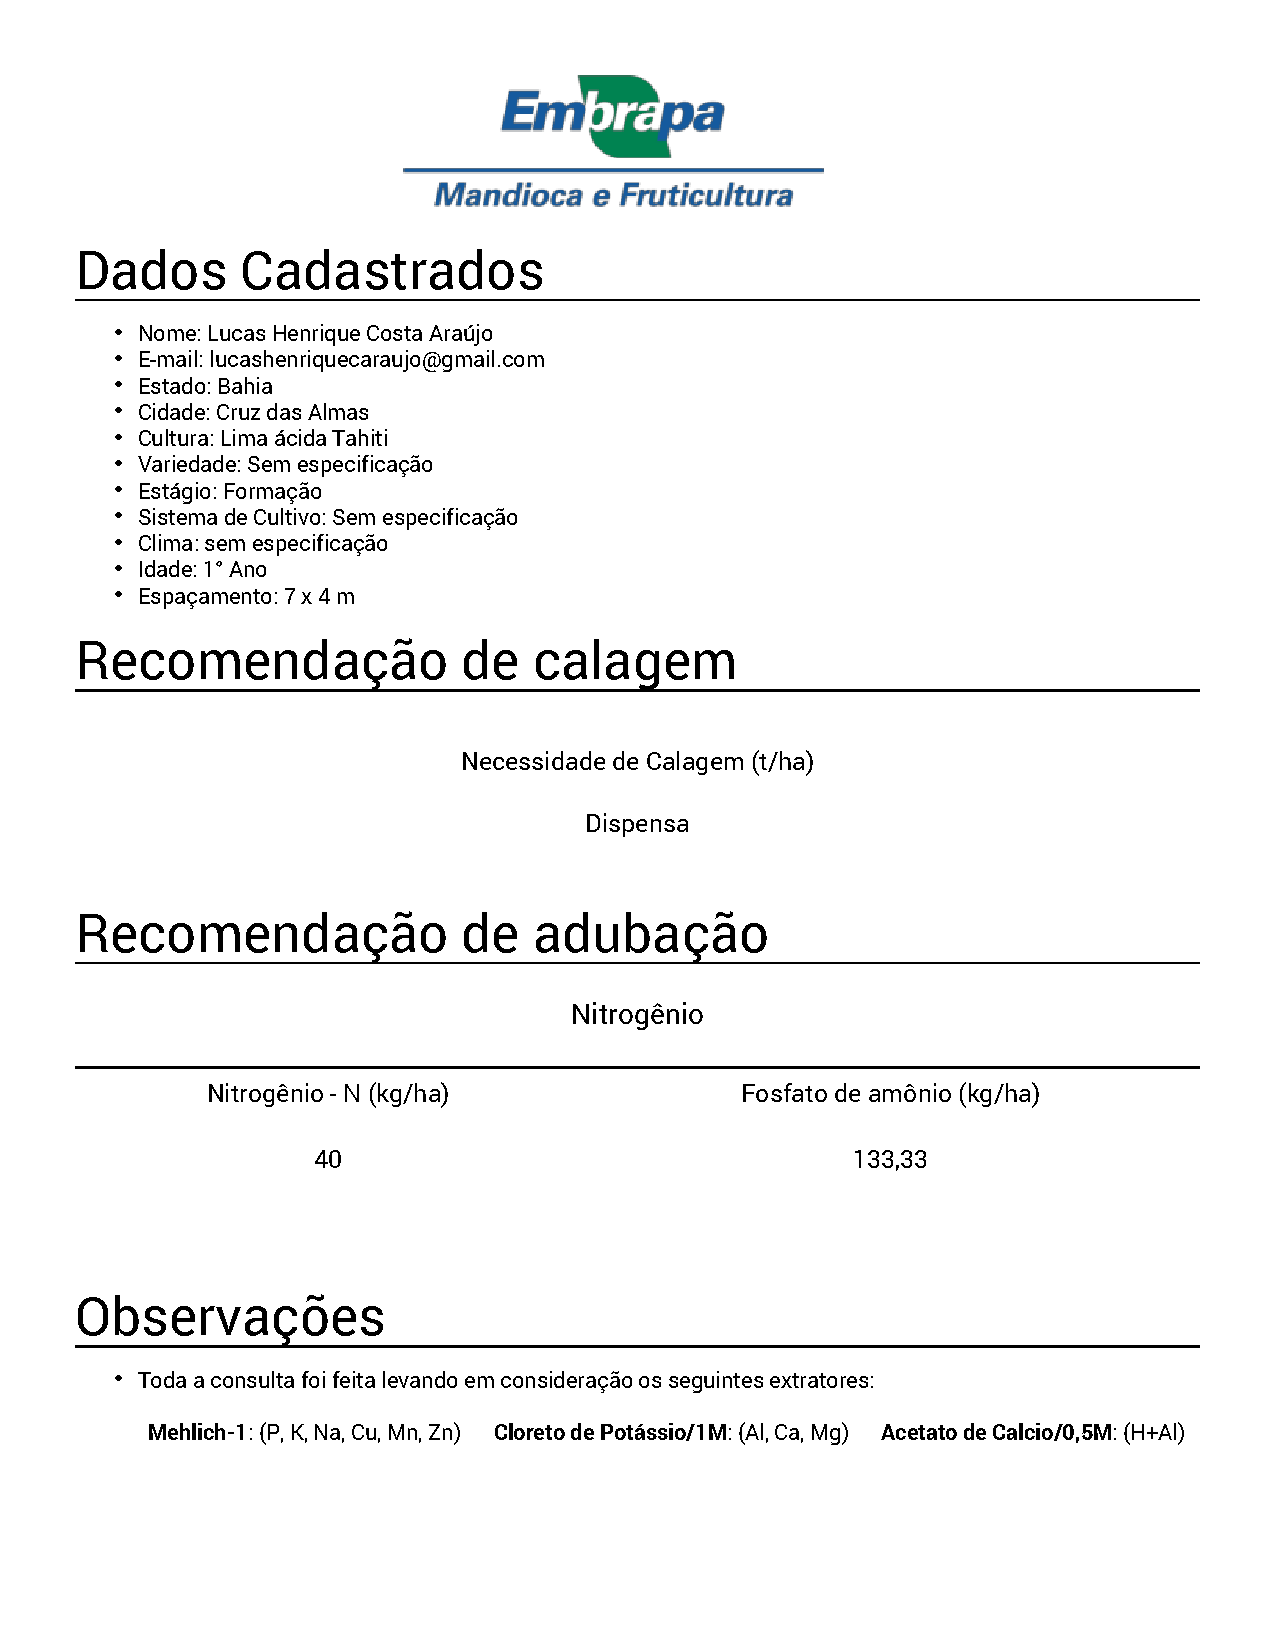
\includepdf[pages=-]{resultadoOriginal1.pdf}
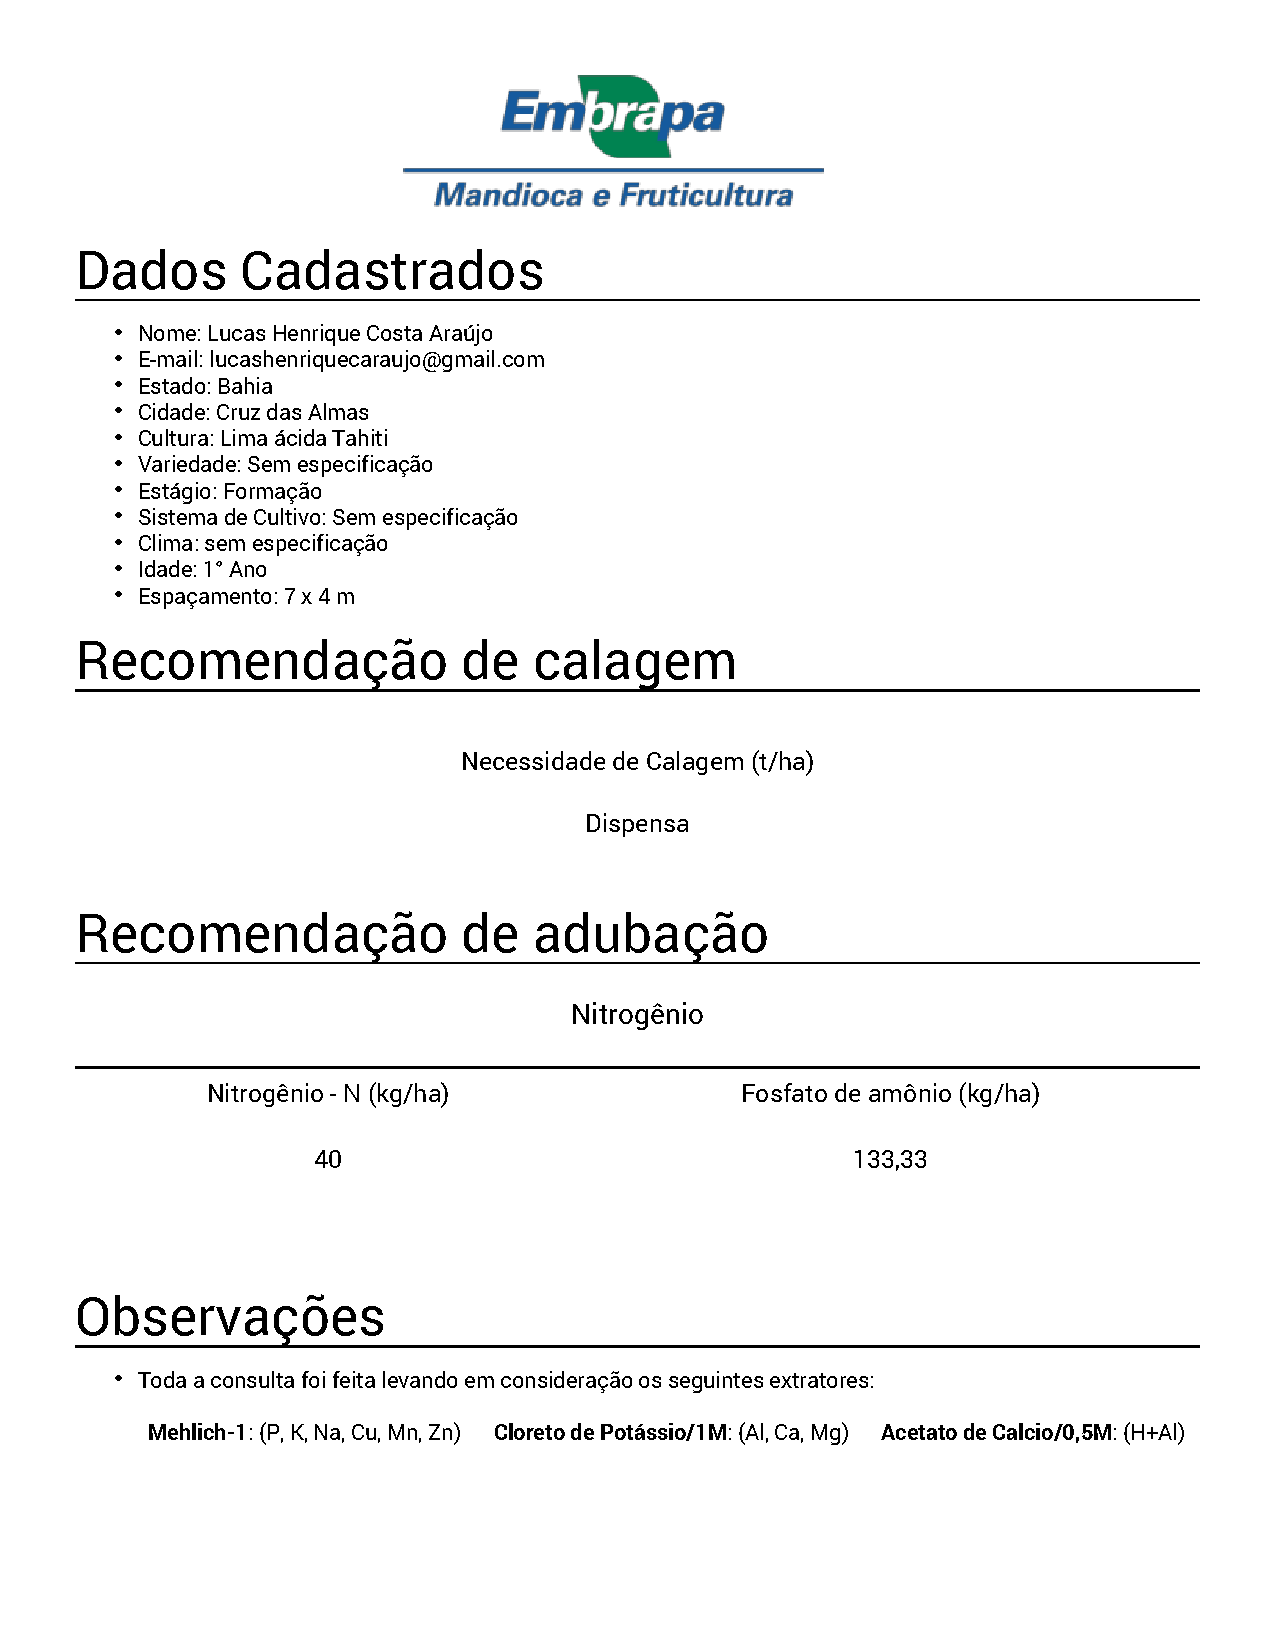
\includepdf[pages=-]{resultadoPredito1.pdf}


\end{document}
